\documentclass[12pt,a4paper]{article}
\usepackage[T2A]{fontenc}
\usepackage[russian]{babel}
\usepackage[utf8]{inputenc}
\usepackage{multirow}
\usepackage{hhline}
\usepackage{indentfirst}
\usepackage[Magistr]{ptvstyle}
\usepackage{graphicx}
\title{Оптимальный алгоритм решения задачи линейного программирования}
\author{студент группы 381306-2 \\ Кочуев А.И.\\ \noindent\rule{5cm}{0.4pt} \\ подпись\\}
\advisor{к.ф.-м.н, доцент \\ Веселов С.И.\\ \noindent\rule{5cm}{0.4pt} \\ подпись}
\chief{д.ф.-м.н., профессор \\ Кузнецов М.И.}
\date{2017}

\begin{document}

\maketitle

\tableofcontents

\newpage


\section*{Введение}
% Не удаляйте следующую строчку!
\addcontentsline{toc}{section}{Введение}
% Не удаляйте следующую строчку!


Линейное программирование - математическая дисциплина, которая обозревает методы решения и теорию задач на поиск максимума и минимума (экстремальных задач) на множествах векторного пространства, размерность которого $n$. Данное пространство задаётся множеством линейных неравенств и уравнений. Линейное программирование - это частный случай выпуклого программирования, которое является частным случаем математического программирования. Многие свойства задач линейного программирования могут быть интерпретированы геометрически, как свойства многоугольников (в двумерном пространстве) и многогранников (в многомерном пространстве).\par
Задача нахождения минимума линейной функции является общей задачей линейного программирования. Эта линейная функция имеет следующий вид:
\[
f(x)=
\sum_{j=1}^n c_{j}x_{j}
= c_{1}x_{1}+c_{2}x_{2}+\dots+c_{n}x_{n}
\]
Если в задаче есть ограничения в форме неравенств, то такая задача называется основной задачей линейного программирования. Она имеет следующую форму:
\[
\begin{aligned}
\min f(x)&=
\sum_{j=1}^n c_{j}x_{j}
= c_{1}x_{1}+c_{2}x_{2}+\dots+c_{n}x_{n} \text{ , при ограничениях:}\\
&\sum_{j=1}^n c_{i,j}x_{j}\geqslant b_{i,j}, i=1,2,\dots,m \text{ , где m - количество ограничений.}\\
&x_{j}, j=1,2,\dots,n \text{ , где n - размерность пространства.}\\
\end{aligned}
\]
Канонической формой задачи линейного программирования является следующая:
\[
\begin{aligned}
\min f(x)&=
\sum_{j=1}^n c_{j}x_{j}
= c_{1}x_{1}+c_{2}x_{2}+\dots+c_{n}x_{n} \text{ , при ограничениях:}\\
&\sum_{j=1}^n c_{i,j}x_{j}= b_{i,j}, i=1,2,\dots,m \text{ , где m - количество ограничений.}\\
&x_{j}, j=1,2,\dots,n \text{ , где n - размерность пространства.}\\
\end{aligned}
\]
то есть ограничения-неравенства заменены ограничениями-равенствами, путём добавления новых переменных.\par
Так же любые задачи линейного программирования более общего вида, то есть содержащие органичения-равенства, ограничения-неравенства и переменные, свободные от ограничений, могут быть приведены к эквивалентным каноническим.\par


%%%%%%%%%%%%%%%%%


\newpage
Рассмотрим некоторые примеры задач линейного программирования:\par
\begin{enumerate}
\item Задача нахождения максимального паросочетания.\par
	В данной задаче необходимо найти максимальное паросочетание в двудольном графе. В форме задачи линейного 		программирования эта задача принимает вид: 
	\[
	\begin{aligned}
	\max f(x)&=
	\sum_{i=1}^n \sum_{j=1}^m x_{i,j} \text{ , при ограничениях:} \\
	&\sum_{i=1}^n x_{i,j} \leqslant 1, j=1,2,\dots,m \text{ , где i - номер вершины в одной доле.}\\
	&\sum_{j=1}^m x_{i,j} \leqslant 1, i=1,2,\dots,n \text{ , где j - номер вершины во второй доле.}\\
	&0 \leqslant x_{i,j} \leqslant 1
	\end{aligned}
	\]
\item Транспортная задача.\par
	Частным случает транспортной задачи является задача о перевозке груза, то есть требуется составить наиболее 		выгодный, то есть самый дешёвый способ доставки. В данной задаче $ c_{i,j}$ - расстояние от $i$-ого склада до $j$-ого завода, $x_{i,j}$ - количество груза, которое перевозится из  $i$-ого склада до $j$-ый завод.($b_{j}$ - потребность в грузе на $j$-ом заводе.$a_{i}$ - количество груза на $i$-ом складе.)
	\[
	\begin{aligned}
	\min f(x)&=
	\sum_{i=1}^n \sum_{j=1}^m x_{i,j} c_{i,j} \text{ , при ограничениях:}\\
	&\sum_{j=1}^m x_{i,j} \leqslant a_{i}, i=1,2,\dots,n \\
	&\sum_{i=1}^n x_{i,j} \geqslant b_{j}, j=1,2,\dots,m \\
	\end{aligned}
	\]
\item Задача об игре с нулевой суммой.\par
	Дана матрица $A$ размерностью $n \times m$. Игрок, который выбирает первым, загадывает число от $1$ до $n$, второй - от $1$ до $m$. После этого они вскрывают свои числа и тот, кто выбирал первым получает $a_{i,j}$ очков ($a_{i,j}$ - элемент матрицы $A$, находящийся в $i$-ой строке и $j$- ом столбце), а второй игрок $(-a_{i,j})$. Требуется найти оптимальную стратегию первого игрока.\par
	Обозначим за $p_{i}$ вероятность того, что первый игрок выбрал число $i$, $c$ - математическое ожидание выигрыша первого игрока в наихудшем случае. Тогда игра с нулевой суммой сводится к задаче линейного программирования:
	\[
	\begin{aligned}
	\max &f( p_{1},\dots, p_{n},c)=c  \text{ , при ограничениях:}\\
	&\sum_{i=1}^n a_{i,j} p_{i}\geqslant c, j=1,2,\dots,m \\
	&0 \leqslant p_{i} \leqslant 1 \\
	&\sum_{i=1}^n p_{i} = 1, i=1,2,\dots,m \\
	\end{aligned}
	\]
\end{enumerate}


%%%%%%%%%%%%%%%%%%%%%%%%%%%%%%%%%%%%%%


В наше время существует множество методов решения задач линейного программирования. Самым популярным из них является симплекс-метод. Этот метод решает задачу линейного программирования, перебирая вершины выпуклого многоугольника (в двумерном пространстве) или выпуклого многогранника (в многомерном пространстве). Хотя, симплекс-метод однозначно решает поставленную перед ним задачу, но делает он это за экспоненциальное время, что является не самым оптимальным.\par 
Поэтому, так как поиск оптимального алгоритма решения задачи линейного программирования является актуальной в наше время задачей, в моей работе был описан и реализован оптимальный, линейный от числа ограничений, алгоритм решения задачи линейного программирования вида:  
\[
\begin{aligned}
	\min\, &ax+by \\
	&a_{i}x+b_{i}y+c_{i} \leqslant 0, i=1,2,\dots,N
\end{aligned}
\]



%%%%%%%%%%%%%%%%%%%%%%%%%%%%%%%%%%%%%%



\newpage
\section{Алгоритм Мегиддо.}
  Метод описан в статье Мегиддо \cite{Megiddo} и в книге \cite{Preparata89}.
  
	Исходную задачу\par
\[
\begin{aligned}
	\min\, & ax+by \\
	&a_{i}x+b_{i}y+c_{i} \leqslant 0, i=1,2,\dots,N
\end{aligned}
\]
можно модифицировать, используя линейные преобразования, которые осуществляются за линейное от числа ограничений-неравенств время $O(n)$, $n$ - число ограничений, взяв $Y=ax+by$ и $X=x$, следующим образом:
\[
\begin{aligned}
	\min\, & Y \\
	&\alpha_{i}X+\beta_{i}Y+c_{i} \leqslant 0, i=1,2,\dots,N
\end{aligned}
\]
где $\alpha_{i}=(a_{i}-(a/b)\beta_{i})$, $\beta_{i}=b_{i}/b$. (Рис.~\ref{ris:main1})\par

\begin{figure}[h]
\center{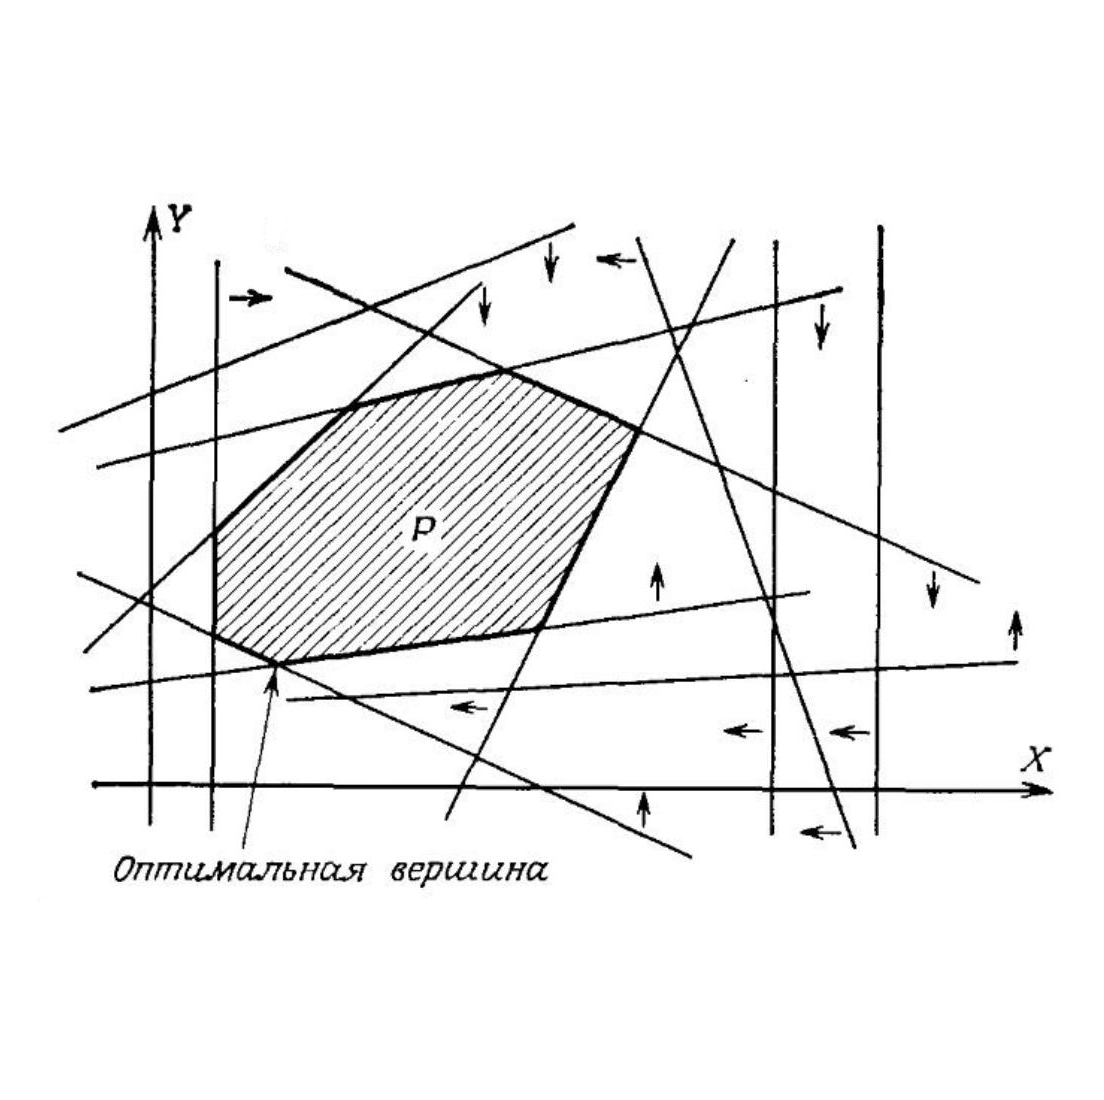
\includegraphics[width=0.5\linewidth]{Images/main1}}
\caption{Многоугольник исходной задачи.}
\label{ris:main1}
\end{figure}


%%%%%%%%%%%%%%%%%%%%%%%%%%%%%%%%%%%%%%%%%%%%


\newpage
В новой, преобразованной, задаче необходимо вычислить наименьшее значение $Y$ на вершинах выпуклого многоугольника $P$ (допустимой области), который определяется этими $n$ ограничениями. Чтобы не строить всю границу $P$, осуществим следующие действия. В зависимости от того, будет ли $\beta_{i}$ нулём, отрицательным или положительным числом, разобьём множество индексов $1,\dots,N$ на подмножества: 
\begin{enumerate}
\item $ I_{0}$, если $\beta_{i} = 0$.\par
Все ограничения с индексами из $ I_{0}$ являются вертикальными прямыми (т.е. параллельными оси Y) и определяют допустимый интервал X следующим образом:
\[
\begin{aligned}
&u_{1}\leqslant X \leqslant u_{2},\\
&u_{1}= \max\{-c_{i}/\alpha_{i}: i\in I_{0}\}\\
&u_{2}=\min \{-c_{i}/\alpha_{i}: i\in I_{0}\}
\end{aligned}
\]
вычисление $u_{1}$ и $u_{2}$ производится за линейное время $O(|I_{0}|)$.\par
\item $ I_{-}$, если $\beta_{i} < 0$.\par
Приняв $\delta_{i}=-(\alpha_{i}/\beta_{i})$ и $\gamma_{i}=-(c_{i}/\beta_{i})$, получаем, что все ограничения из $I_{-}$ имеют вид:
\[
Y\geqslant\delta_{i}X+\gamma_{i},  i\in I_{-},
\]
они, вместе взятые, определяют кусочно-линейную, выпуклую вверх функцию $F_{-}(X)$ вида:
\[
F_{-}(X)=\max_{ i\in I_{-}}(\delta_{i}X+\gamma_{i}),
\]
данное преобразование производится за линейное время $O(|I_{-}|)$.\par
\item $ I_{+}$, если $\beta_{i} > 0$. \par
Приняв $\delta_{i}=-(\alpha_{i}/\beta_{i})$ и $\gamma_{i}=-(c_{i}/\beta_{i})$, получаем, что все ограничения из $I_{+}$ имеют вид:
\[
Y\leqslant\delta_{i}X+\gamma_{i},  i\in I_{+},
\]
они, вместе взятые, определяют кусочно-линейную, выпуклую вверх функцию $F_{+}(X)$ вида:
\[
F_{+}(X)=\min_{ i\in I_{+}}(\delta_{i}X+\gamma_{i}),
\]
данное преобразование производится за линейное время $O(|I_{+}|)$.\par
\end{enumerate}



После таких линейных преобразований и такого разделения, получаем неравенство 
\[
F_{-}(X)\leqslant Y\leqslant F_{+}(X),
\]
а так как решается задача линейного программирования на определение минимума функции, при заданных ограничениях, то $F_{-}(X)$ и является нашей целевой функцией, а по свойству выпуклой функции её локальный минимум будет являтся и глобальным, и задача преобразуется в следующую:
\[
\begin{aligned}
	\min&  F_{-}(X) \\
	&F_{-}(X)\leqslant F_{+}(X),\\
	&u_{1}\leqslant X\leqslant u_{2}.
\end{aligned}
\]
Новая ситуация изображена на (Рис.~\ref{ris:main2}), где показаны связи между $u_{1}$, $u_{2}$, $F_{-}(X)$, $F_{+}(X)$ и границей многоугольника $P$.\par

\begin{figure}[h]
\center{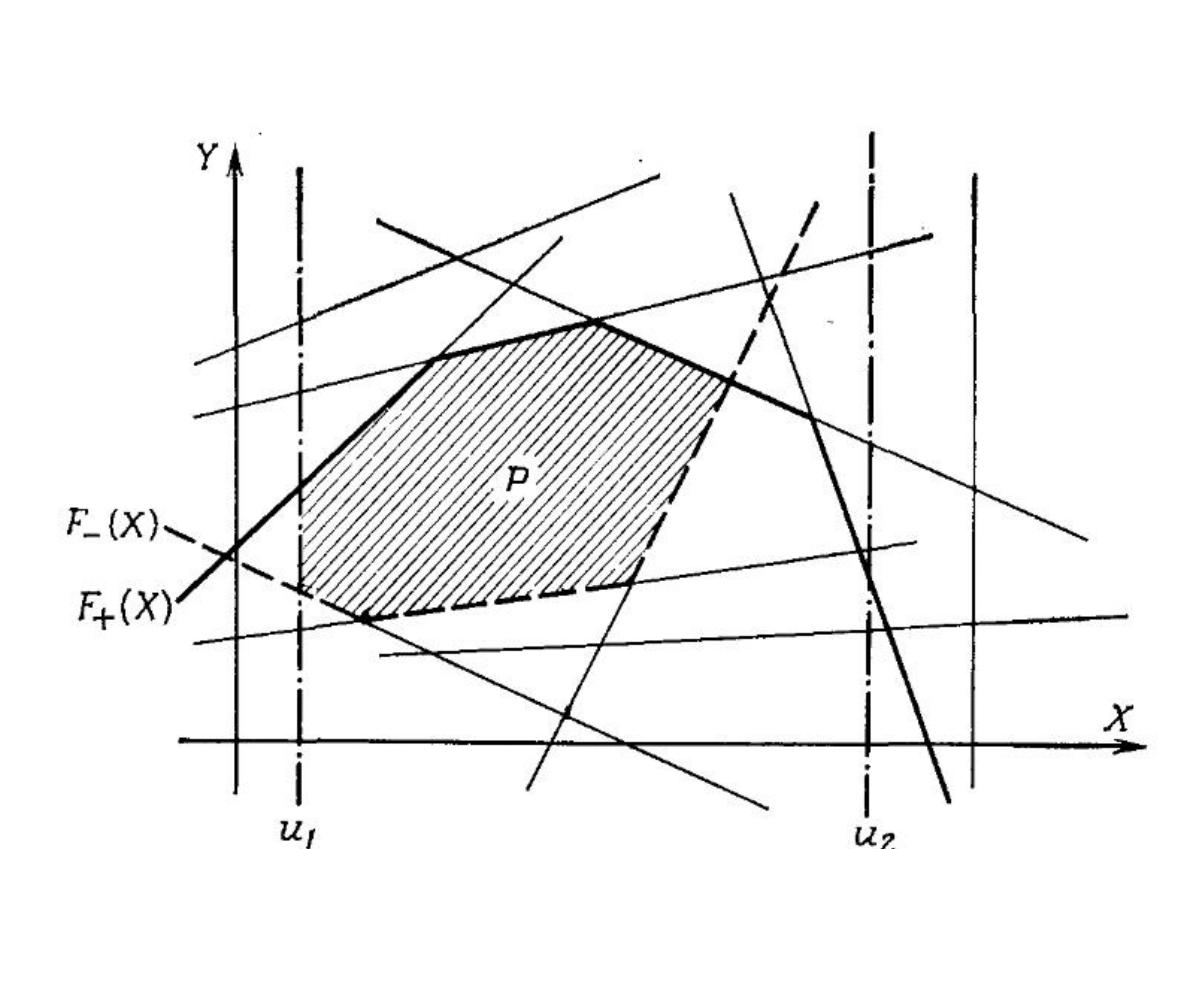
\includegraphics[width=0.625\linewidth]{Images/main2}}
\caption{Многоугольник задачи минимизации $ F_{-}(X)$.}
\label{ris:main2}
\end{figure}

Элементарной операцией, используемой в этом методе, является вычисление функций $F_{-}(X')$, $F_{+}(X')$ и их наклонов по обе стороны от заданного значения $X'\in X$. Обозначим через $f_{-}^{(L)}(X')$ и $f_{-}^{(R)}(X')$ наклоны  $F_{-}(X')$ слева и справа от $ X'$ соответственно. Аналогично для $F_{+}(X')$ : $f_{+}^{(L)}(X')$ и $f_{+}^{(R)}(X')$. Покажем теперь, что эту операцию, названную вычислением функций $F_{-}(X')$, $F_{+}(X')$, $f_{-}^{(L)}(X')$ и $f_{-}^{(R)}(X')$, можно выполнить за время $O( n)$.\par
\begin{enumerate}
\item Для $F_{-}(X)$, имеем выражение:
\[
F_{-}(X')=\max_{ i\in I_{-}}(\delta_{i}X'+\gamma_{i}),
\]
которое можно вычислить за время пропорциональное $| I_{-}|=O( n)$.
\begin{enumerate} 
\item Если существует только одно значение $i$, равное $i_{0}$, на котором достигается $F_{-}(X')$, то $f_{-}^{(L)}(X')=f_{-}^{(R)}(X')=\delta_{i_{0}}$.
\item Если существует два таких значения $i_{1}$ и $i_{2}$, то $f_{-}^{(L)}(X')=\min (\delta_{i_{1}},\delta_{i_{2}})$ и $f_{-}^{(R)}(X')=\max (\delta_{i_{1}},\delta_{i_{2}})$, так как  $F_{-}(X)$ выпукла вниз.\par
\end{enumerate}
\item Для $F_{+}(X)$, имеем выражение:
\[
F_{+}(X')=\min_{ i\in I_{+}}(\delta_{i}X'+\gamma_{i}),
\]
которое можно вычислить за время пропорциональное $| I_{+}|=O( n)$. 
\begin{enumerate}
\item Если существует только одно значение $i$, равное $i_{0}$, на котором достигается $F_{+}(X')$, то $f_{+}^{(L)}(X')=f_{+}^{(R)}(X')=\delta_{i_{0}}$.
\item Если существует два таких значения $i_{1}$ и $i_{2}$, то $f_{+}^{(L)}(X')=\max (\delta_{i_{1}},\delta_{i_{2}})$ и $f_{+}^{(R)}(X')=\min (\delta_{i_{1}},\delta_{i_{2}})$, так как  $F_{+}(X)$ выпукла вверх.\par
\end{enumerate}
\end{enumerate}

Очевидна справедливость утверждения,что для любого $X'\in [u_{1},u_{2}]$ можно получить один из следующих результатов за время $O(n)$:
\begin{enumerate}
\item $X'$ недопустимо, а задача не имеет решений.
\item $X'$ недопустимо, но известно, по какую сторону от $X'$ (слева или справа) могут лежать все допустимые значения $X$.
\item $X'$ допустимо, и известно, по какую сторону от $X'$ лежит минимум $F_{-}(X)$.
\item $X'$ доставляет минимум функции $F_{-}(X)$.
\end{enumerate}


%%%%%%%%%%%%%%%%%%%%%%%%%%%%%%%%

\newpage
\begin{enumerate}
\item Если функция $H(X)=F_{-}(X)-F_{+}(X)>0$  в точке $X'$, то $X'$ недопустимо. Рассматривая наклоны функций $F_{-}(X)\ \text{и }\ F_{+}(X)$ в точке $X'$, имеем: \par 
\begin{enumerate}
\item Eсли $f_{-}^{(L)}(X')>f_{+}^{(L)}(X')$, то $H(X)$ возрастает в $X'$, и допустимые значения $X$ могут располагаться только слева от $X'$. (Рис.~\ref{ris:tangens2}, a)
\item Если $f_{-}^{(R)}(X')<f_{+}^{(R)}(X')$, то $H(X)$ убывает в $X'$, и допустимые значения $X$ могут располагаться только справа от $X'$.(Рис.~\ref{ris:tangens2}, b)
\item Если $f_{-}^{(L)}(X')\leqslant f_{+}^{(L)}(X')$ и $f_{-}^{(R)}(X')\geqslant f_{+}^{(R)}(X')$, то $H(X)$ достигает минимума на $X'$ - задача неразрешима.(Рис.~\ref{ris:tangens2}, c, d)\par
\end{enumerate}

\begin{figure}[h!]
\begin{minipage}[h!]{0.45\linewidth}
\center{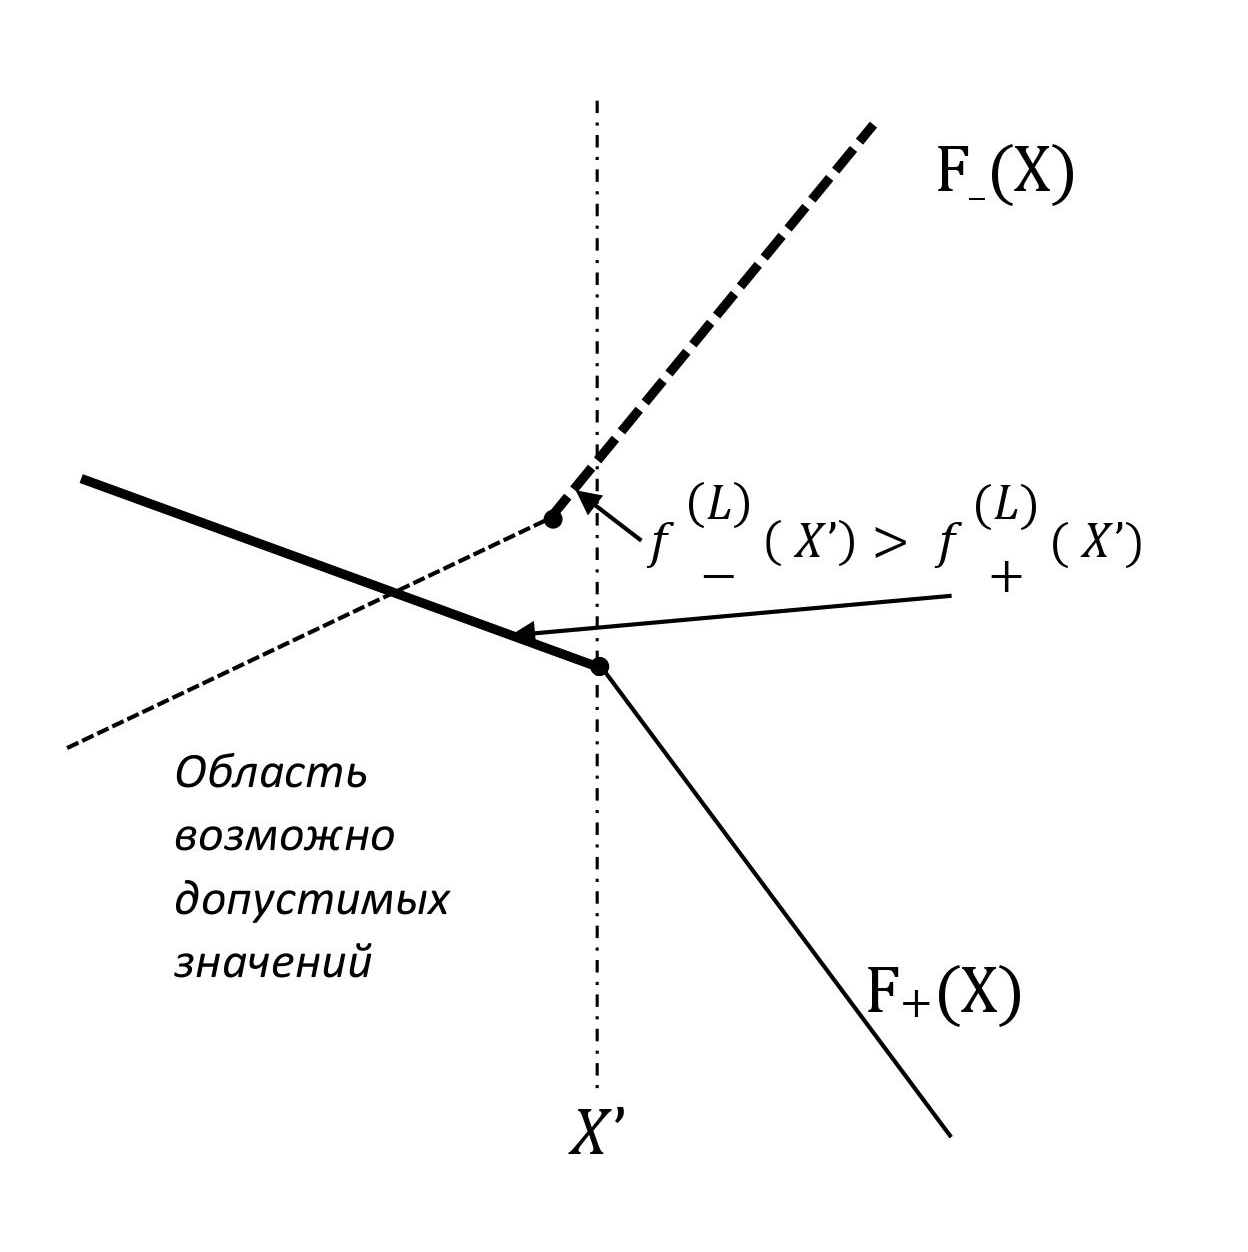
\includegraphics[width=1\linewidth]{Images/fL-fL+} \\ a)}
\end{minipage}
\hfill
\begin{minipage}[h!]{0.45\linewidth}
\center{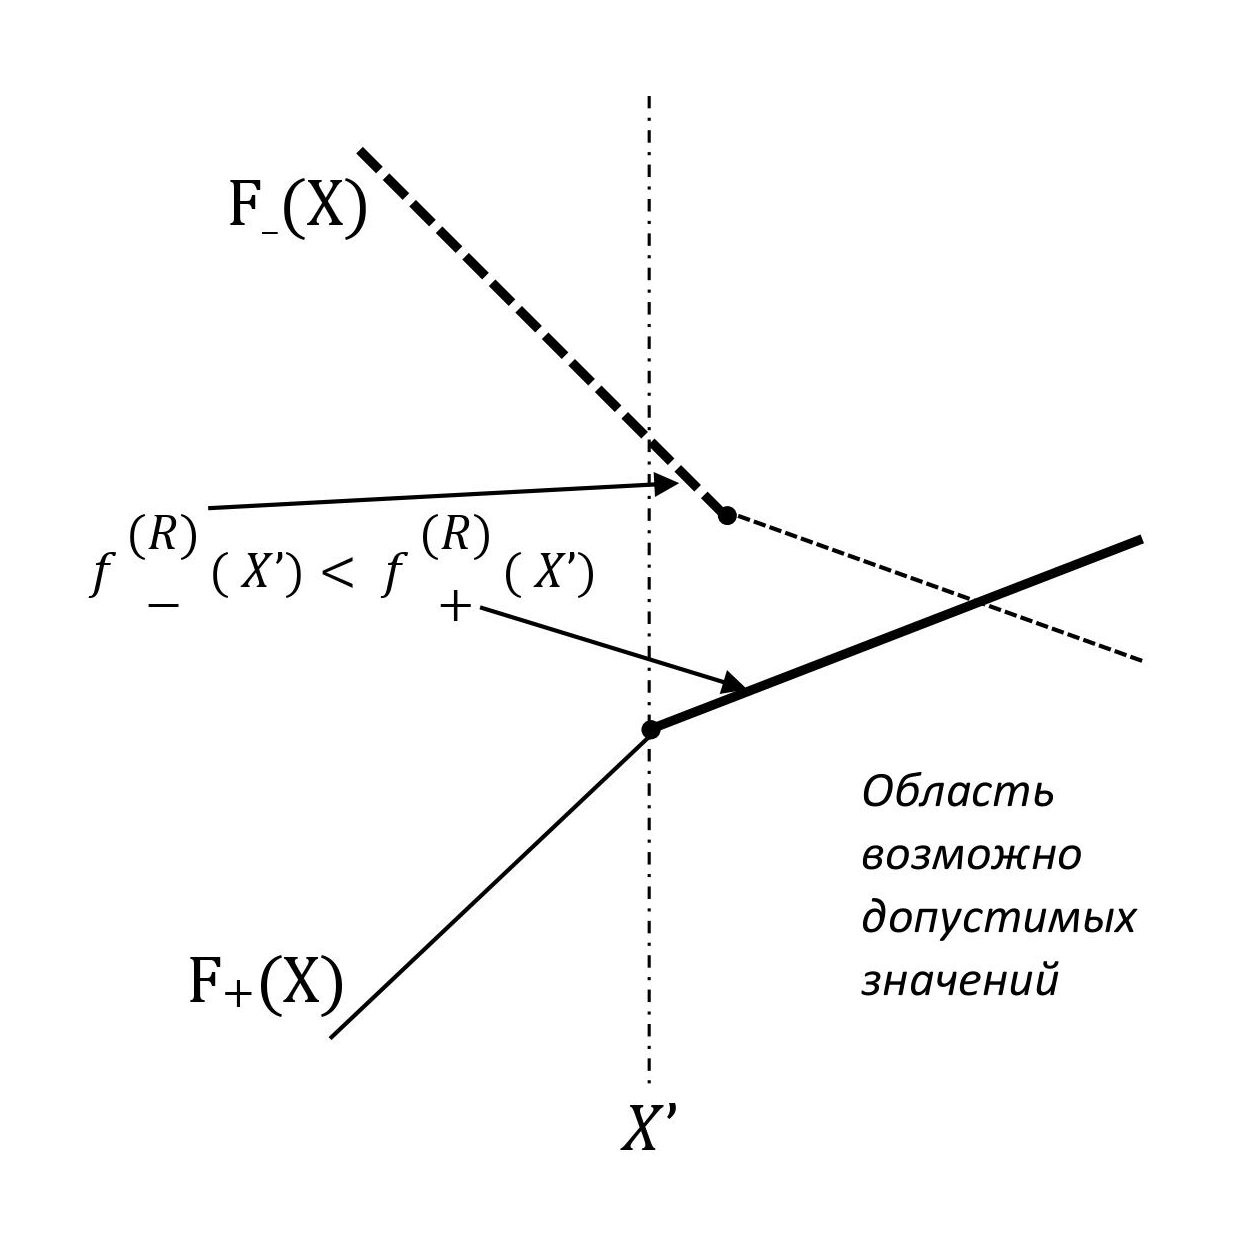
\includegraphics[width=1\linewidth]{Images/fR-fR+} \\ b)}
\end{minipage}
\hfill
\begin{minipage}[h!]{0.45\linewidth}
\center{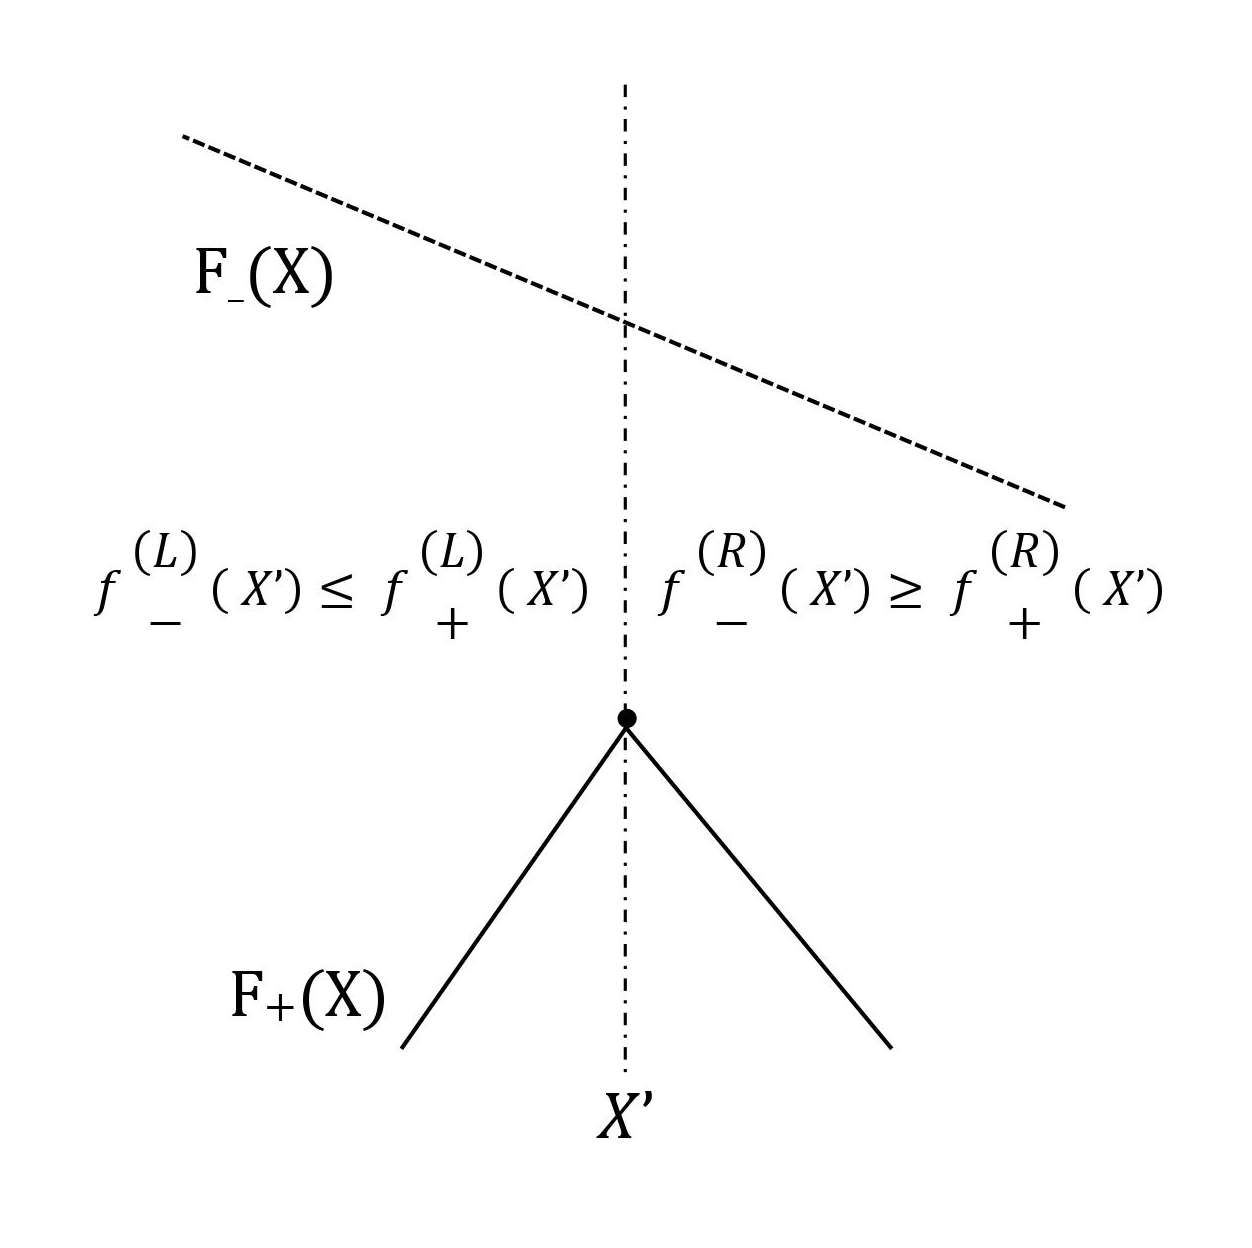
\includegraphics[width=1\linewidth]{Images/fL-fL+fR-fR+1} \\ c)}
\end{minipage}
\hfill
\begin{minipage}[h!]{0.45\linewidth}
\center{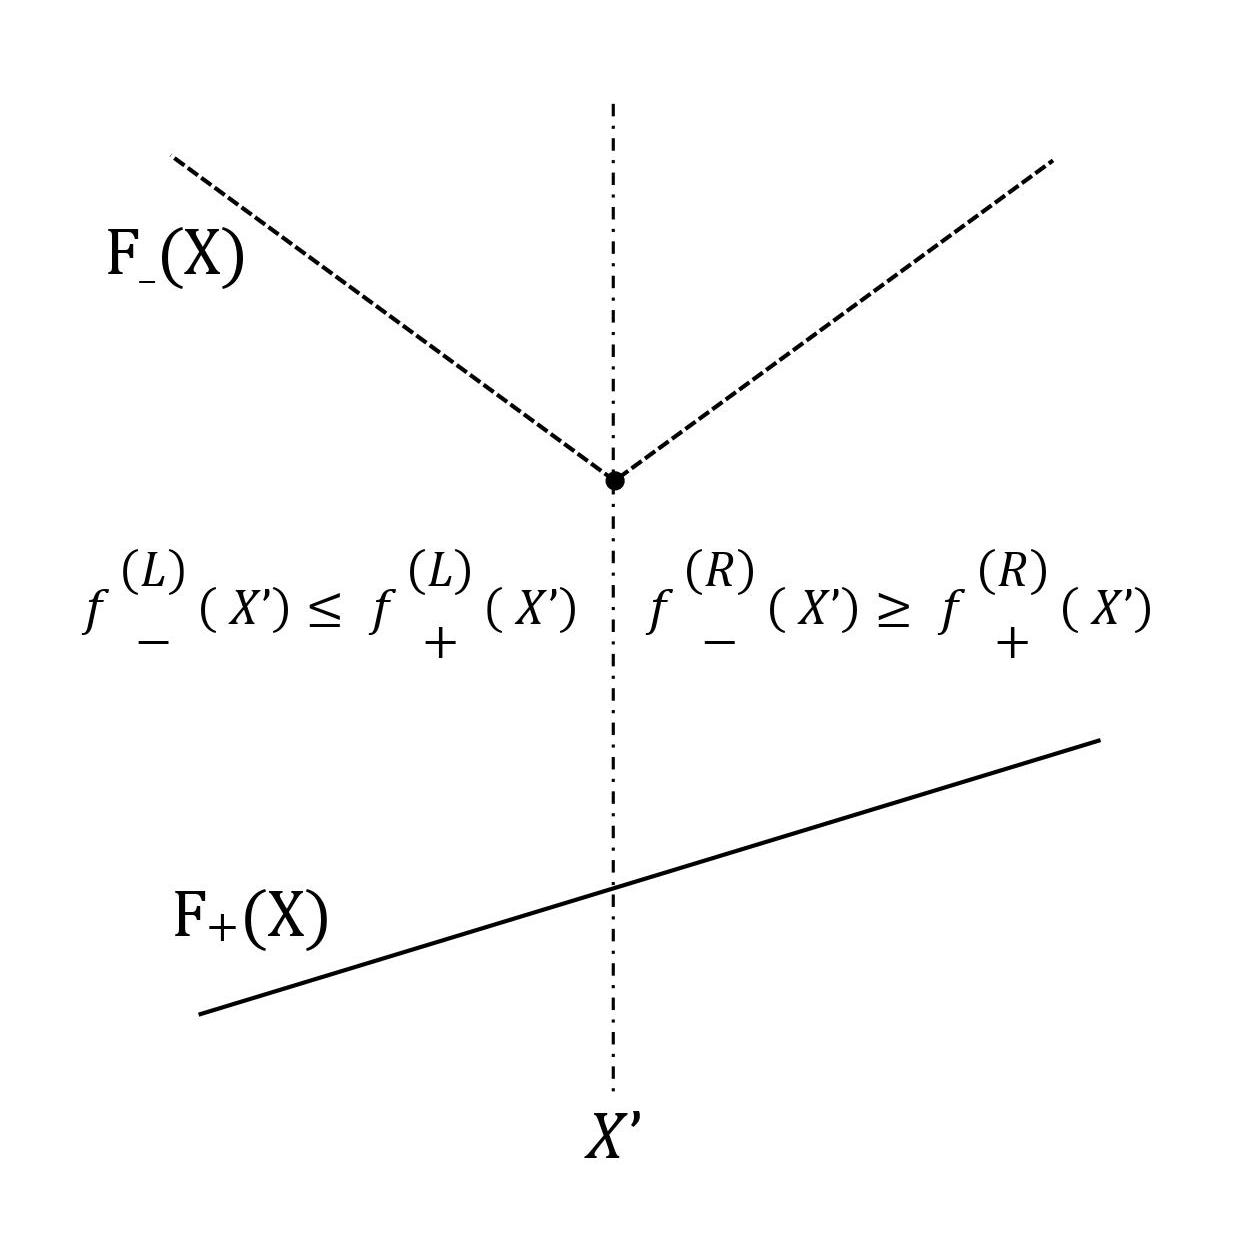
\includegraphics[width=1\linewidth]{Images/fL-fL+fR-fR+2} \\ d)}
\end{minipage}
\caption{$H(X')>0$.}
\label{ris:tangens2}
\end{figure}


%%%%%%%%%%%%%%%%%%%%%%%%%%%%%%%%%%%%%%%%%%%%%%%%%%%%%%%%


\newpage
\itemЕсли функция $H(X') = F_{-}(X')-F_{+}(X')\leqslant 0$, то есть $X'$ - допустимо. Для определения области нахождения минимума достаточно обратить внимание на  поведение функции  $F_{-}(X)$, выпуклой вниз, её правых и левых наклонов, $f_{-}^{(R)}(X)$ и $f_{-}^{(L)}(X)$, относительно  $X'$.\par
\begin{enumerate}
\item Если $f_{-}^{(R)}(X')\geqslant f_{-}^{(L)}(X')>0$, то область где находится минимум располагается слева от  $X'$. (Рис.~\ref{ris:minimum2}, a)\par
\item Если $f_{-}^{(L)}(X')\leqslant f_{-}^{(R)}(X')<0$, то область где находится минимум располагается справа от  $X'$. (Рис.~\ref{ris:minimum2}, b)\par
\item Если $f_{-}^{(R)}(X')= f_{-}^{(L)}(X')=0$, то минимум достигается на этом отрезке. (Рис.~\ref{ris:minimum2}, c)\par
\item Если $f_{-}^{(R)}(X')>0 ,f_{-}^{L)}(X')<0$, то минимум достигается в $X'$. (Рис.~\ref{ris:minimum2}, d)\par
\end{enumerate}

\begin{figure}[h!]
\begin{minipage}[h!]{0.4\linewidth}
\center{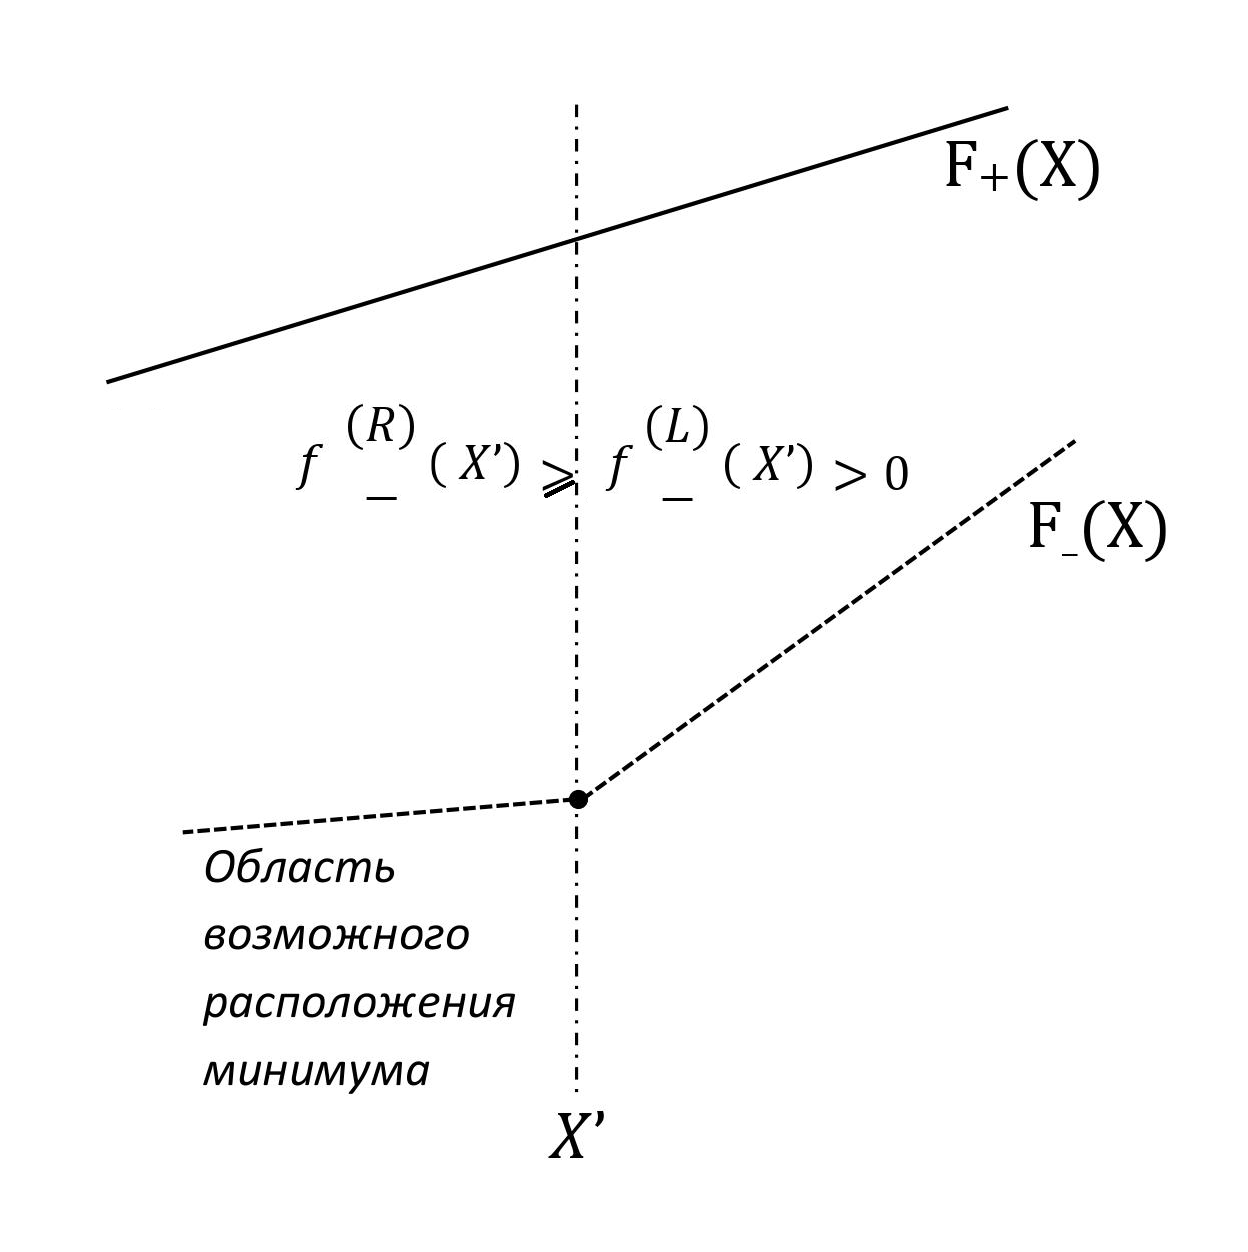
\includegraphics[width=1\linewidth]{Images/fL-fR-02} \\ a)}
\end{minipage}
\hfill
\begin{minipage}[h!]{0.4\linewidth}
\center{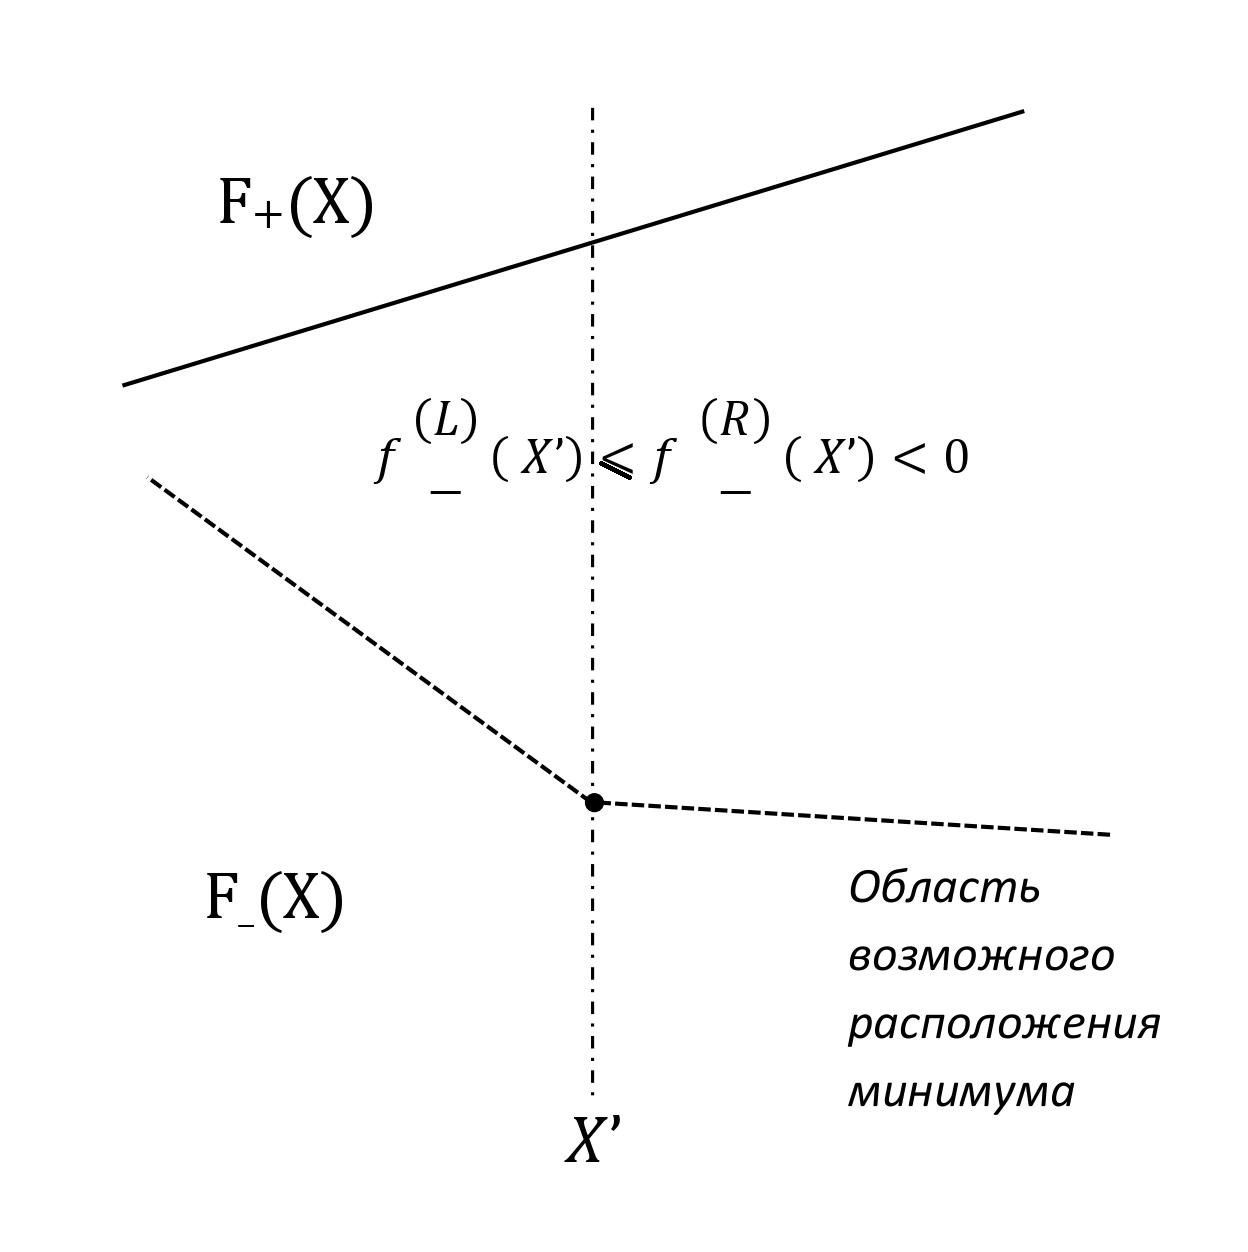
\includegraphics[width=1\linewidth]{Images/fL-fR-01} \\ b)}
\end{minipage}
\hfill
\begin{minipage}[h!]{0.4\linewidth}
\center{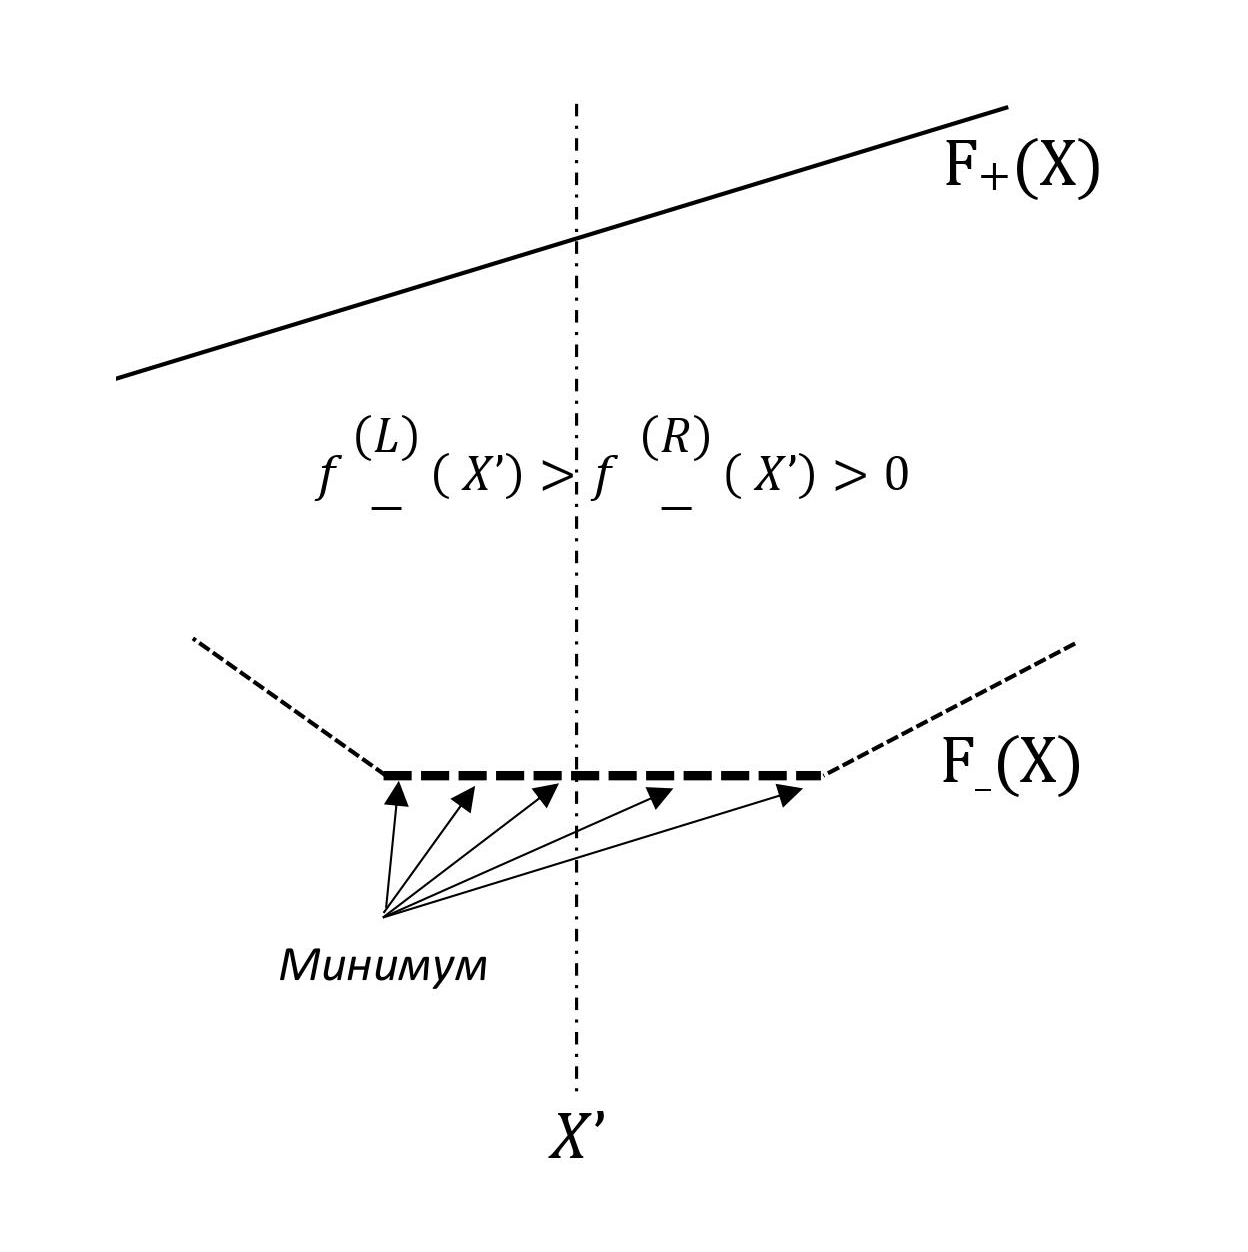
\includegraphics[width=1\linewidth]{Images/fL-fR-03} \\ c)}
\end{minipage}
\hfill
\begin{minipage}[h!]{0.4\linewidth}
\center{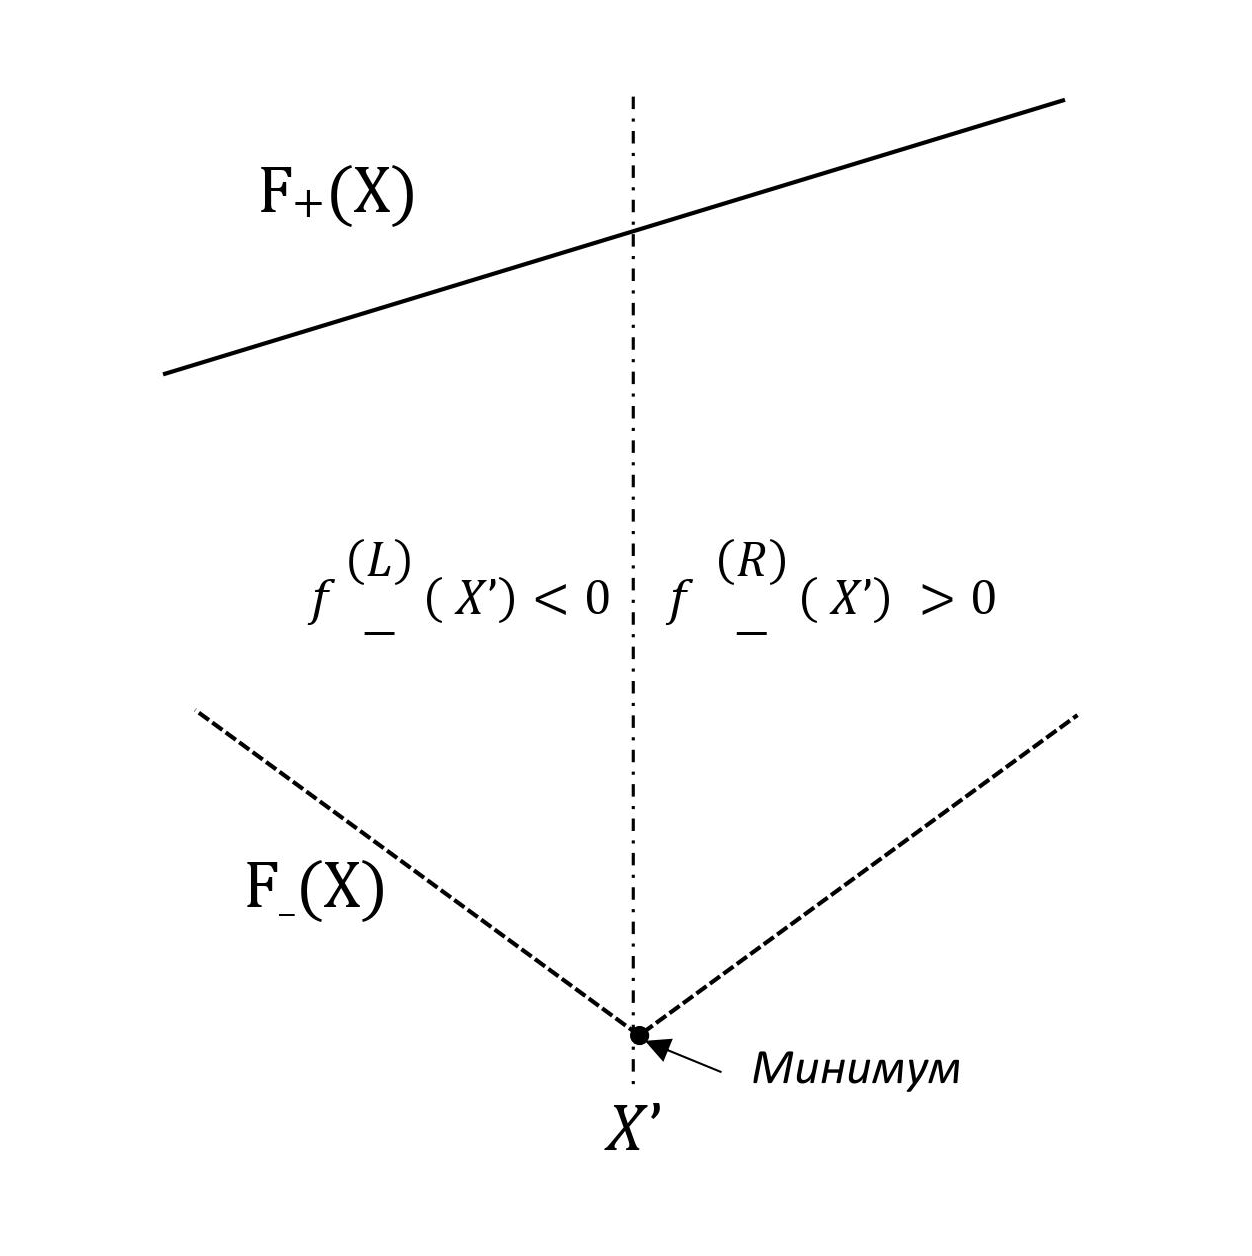
\includegraphics[width=1\linewidth]{Images/fL-fR-0} \\ d)}
\end{minipage}
\caption{$H(X')\leqslant 0$.}
\label{ris:minimum2}
\end{figure}
\end{enumerate}


%%%%%%%%%%%%%%%%%%%%%%%%%%%%%%%%%%%%%%%%%%%%%%%%%%%%%%%%%


\newpage
Получается,что общий принцип заключается в том, что необходимо взять такую абсциссу  $X'$, в которой производится вычисление, чтобы алгоритм либо сразу выдал результат, либо можно было бы отбросить некоторую фиксированную долю $\alpha$ от числа активных ограничений, причём каждое удаляемое ограничение, не должно содержать крайних вершин.  Если мы получаем такой результат, то после $log_{1/(1-\alpha)}N$ шагов мощность множества ограничений-неравенств сокращается настолько, что дальнейшие вычисления можно произвести напрямую. При такой последовательности действий, можно предположить, что на $i$-ом шаге число ограничений не превзойдёт некоторой величины $(1-\alpha)^{i-1}N$, и требуемые вычисления завершатся за время, не превосходящее $K(1-\alpha)^{i-1}N$, где $K$ - некоторая константа. Отсюда получаем, что суммарное время работы $T(N)$ можно оценить сверху следующим неравенством:
\[
\ T(N)\leqslant
\sum_{i=1}^{log_{1/(1-\alpha)}N}
\ K(1-\alpha)^{i-1}N
\ < \frac{KN}{\alpha}
\]
то есть время работы линейно зависит от N, что является оптимальным. Остаётся показать получение величины $\alpha = \frac{1}{4}$.\par
На первом шаге алгоритма, после произведения линейных преобразований множество индексов $1,\dots,N$ разбивается на подмножества:$I_{0}$, $I_{-}$ и $I_{+}$ по принципу описанному в самом начале. Пусть $|I_{-}|+|I_{+}|=M$. Теперь разобьём каждое из множеств  $I_{-}$ и $I_{+}$ на пары ограничений, допускается что по одному ограничению в каждом из множеств останется без пары. Далее исключаем одно из ограничений из пары по описанным ниже правилам. \par

\newpage
\begin{enumerate}
\item Допустим $i,j \in I_{-}$, тогда: \par
\begin{enumerate}
\item Если $\delta_{i}=\delta_{j}$, то получаются параллельные прямые, и одну из них можно сразу удалить, а именно ту, у которой значение $\gamma$ меньше. То есть, если $\gamma_{i}\leqslant \gamma_{j}$ тогда ограничение с номером $i$ можно удалить. (Рис.~\ref{ris:down}, d)

\item Если $\delta_{i}\not=\delta_{j}$, то имеем 3 случая:
\begin{enumerate}
\item Если $X_{ij}<u_{1}$, то удаляем ограничение, у которого значение $\delta$ меньше. (Рис.~\ref{ris:down}, a)
\item Если $X_{ij}>u_{2}$, то удаляем ограничение, у которого значение $\delta$ больше. (Рис.~\ref{ris:down}, b)
\item Если $u_{1}\leqslant X_{ij}\leqslant u_{2}$, то оставляем оба ограничения. (Рис.~\ref{ris:down}, c)
\end{enumerate}
\end{enumerate}

\begin{figure}[h!]
\begin{minipage}[h!]{0.4\linewidth}
\center{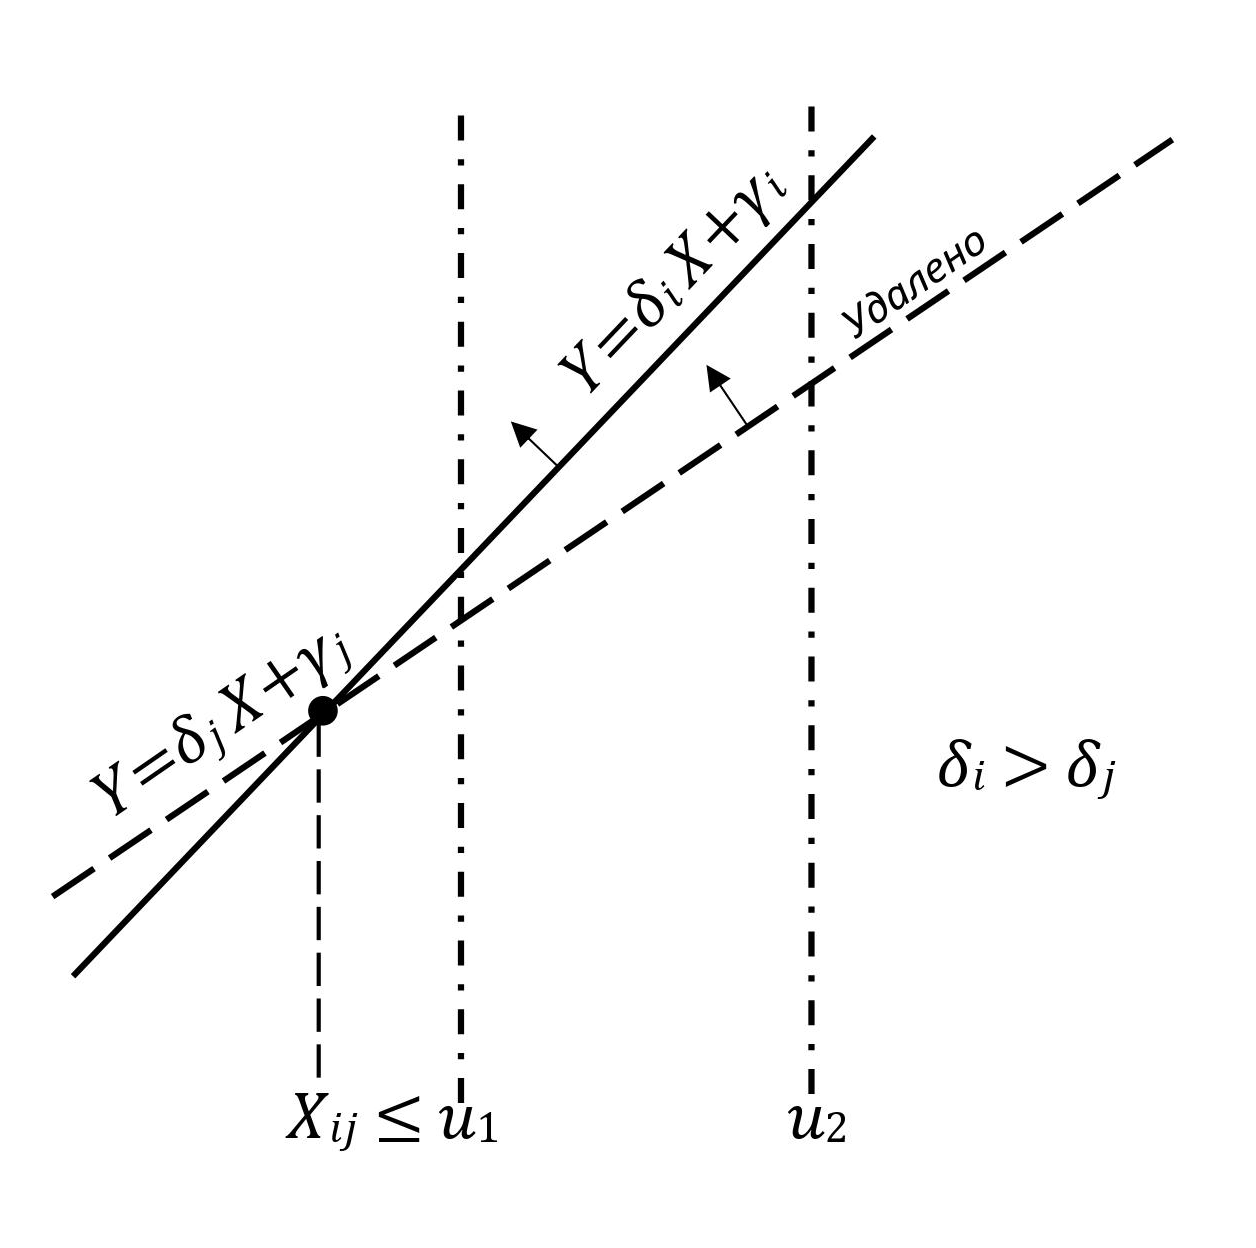
\includegraphics[width=1\linewidth]{Images/du1} \\ a)}
\end{minipage}
\hfill
\begin{minipage}[h!]{0.4\linewidth}
\center{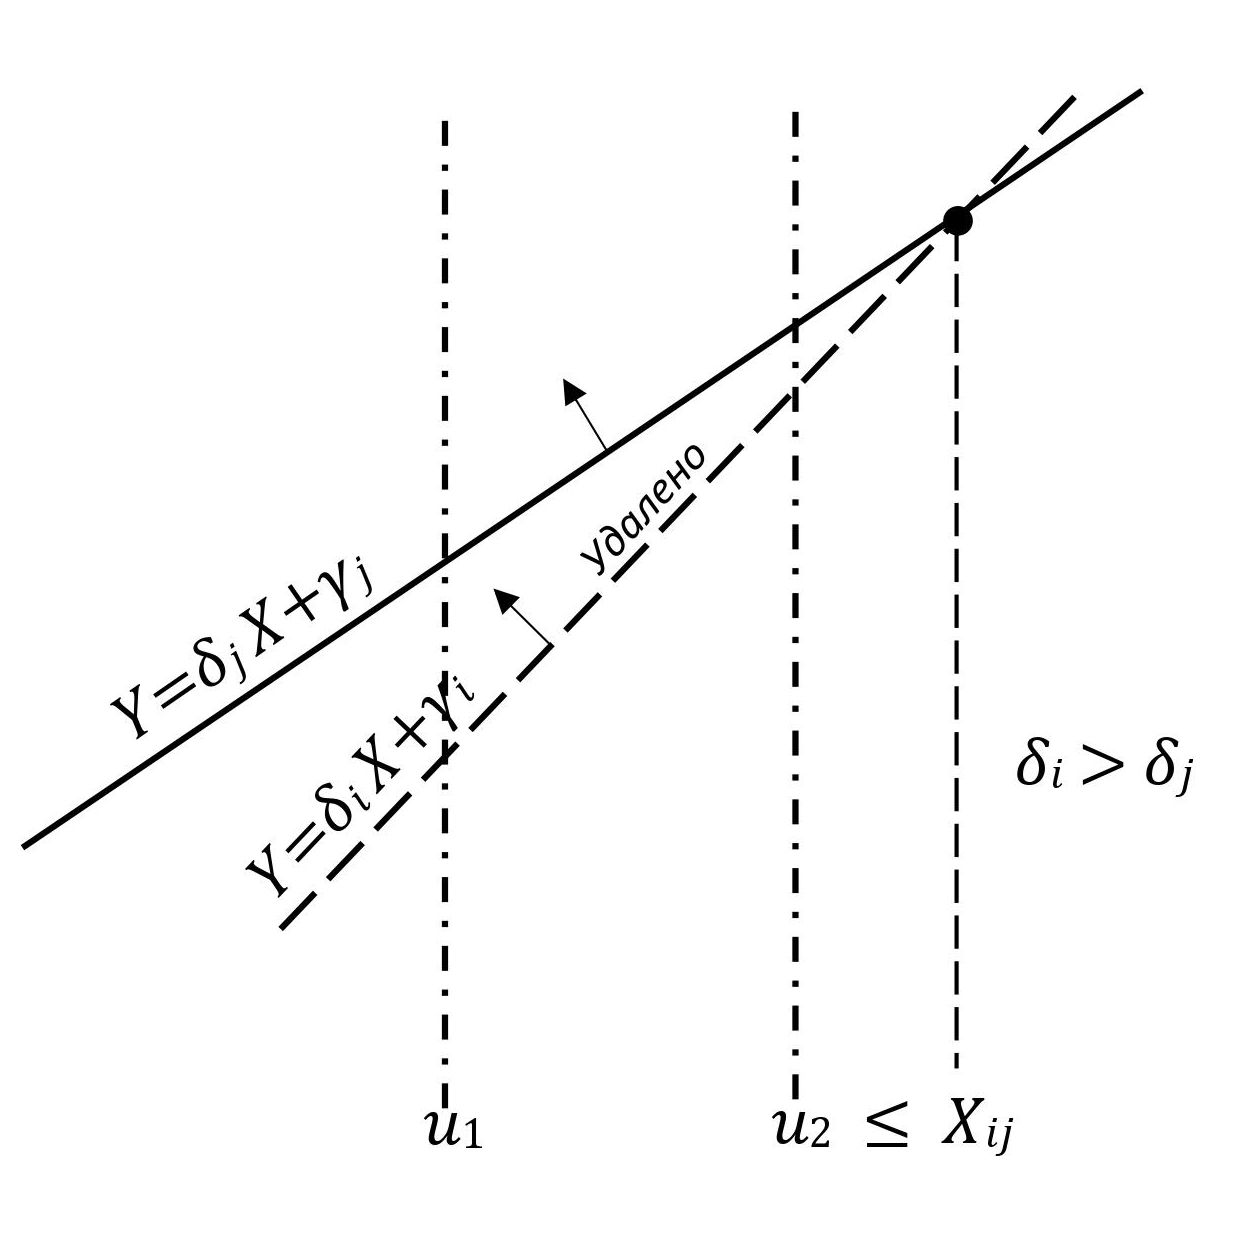
\includegraphics[width=1\linewidth]{Images/du2} \\ b)}
\end{minipage}
\hfill
\begin{minipage}[h!]{0.4\linewidth}
\center{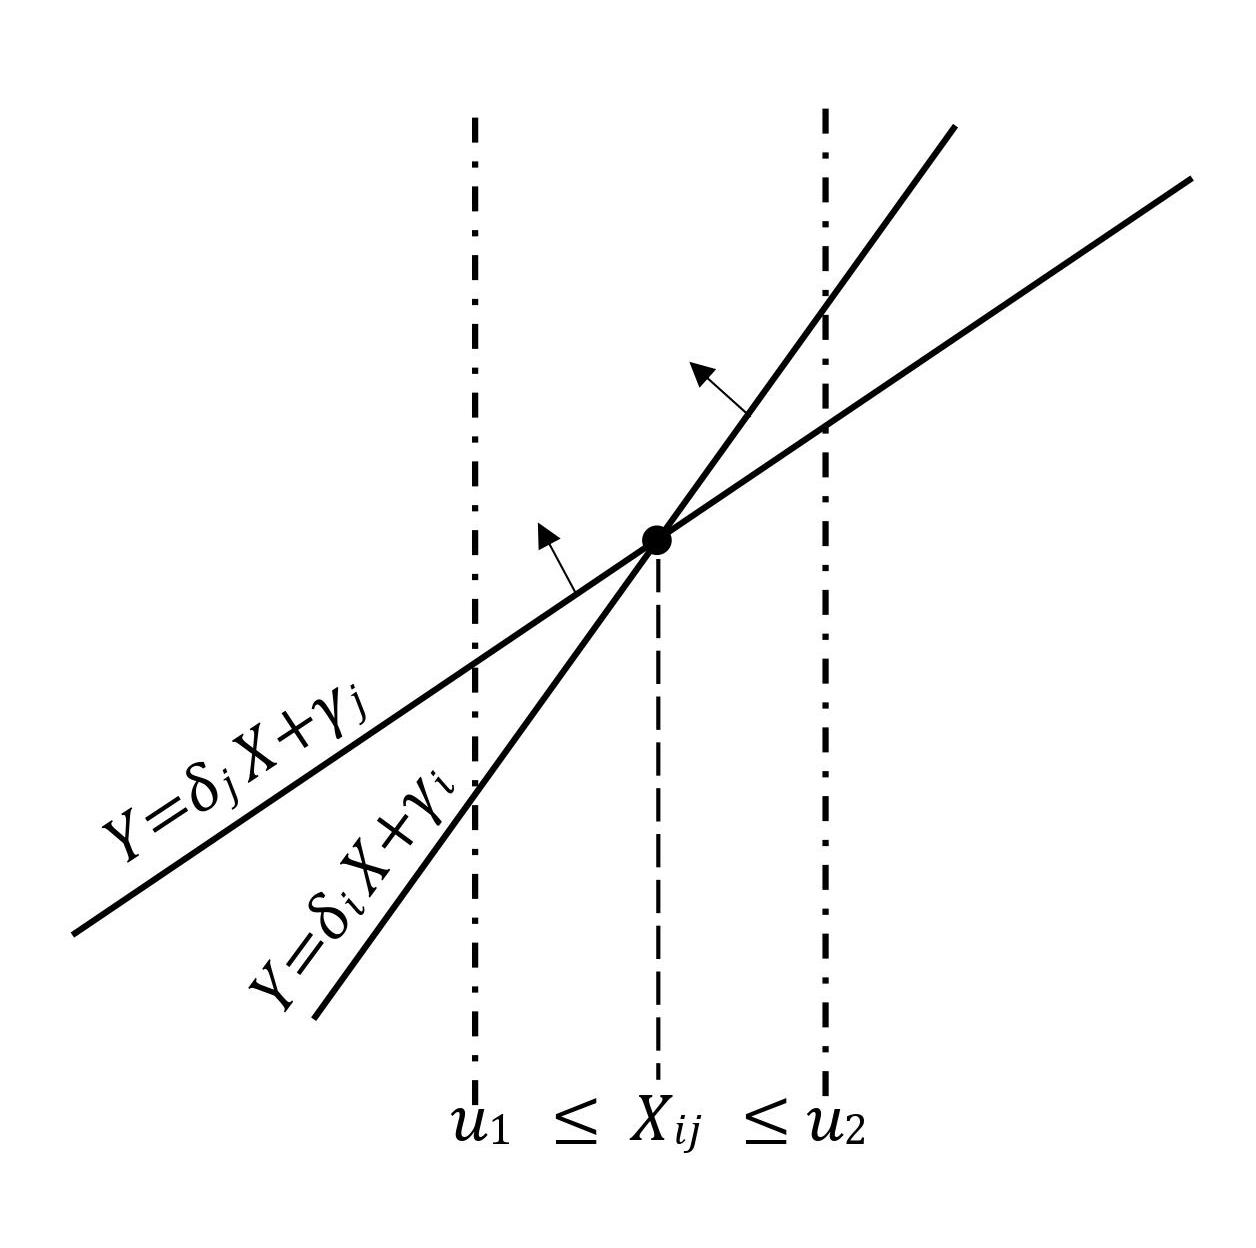
\includegraphics[width=1\linewidth]{Images/du1u2} \\ c)}
\end{minipage}
\hfill
\begin{minipage}[h!]{0.4\linewidth}
\center{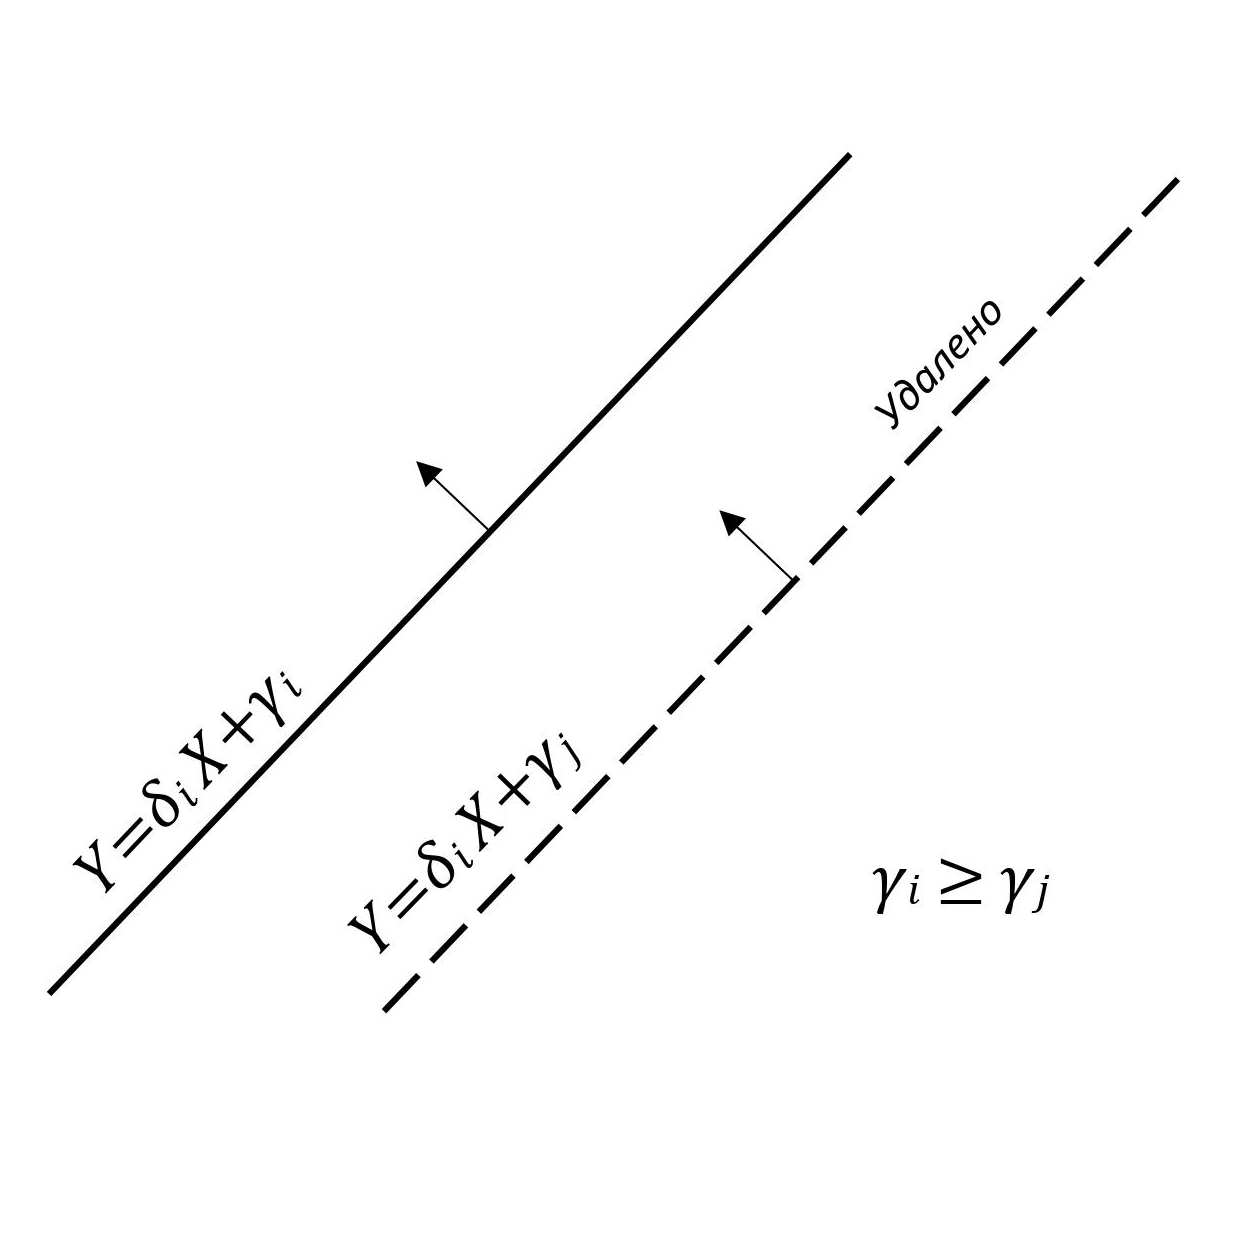
\includegraphics[width=1\linewidth]{Images/dp} \\ d)}
\end{minipage}
\caption{$i,j \in I_{-}$.}
\label{ris:down}
\end{figure}


%%%%%%%%%%%%%%%%%%%%%%%%%%%%%%%%%%%%%%%%%%%%%%%%%%%%%


\newpage
\item Допустим $i,j \in I_{+}$, тогда: \par
\begin{enumerate}
\item Если $\delta_{i}=\delta_{j}$, то получаются параллельные прямые, и одну из них можно сразу удалить, а именно ту, у которой значение $\gamma$ больше. То есть, если $\gamma_{i}\leqslant \gamma_{j}$ тогда ограничение с номером $j$ можно удалить. (Рис.~\ref{ris:up}, d)
\item Если $\delta_{i}\not=\delta_{j}$, то имеем 3 случая:
\begin{enumerate}
\item Если $X_{ij}<u_{1}$, то удаляем ограничение, у которого значение $\delta$ больше. (Рис.~\ref{ris:up}, a)
\item Если $X_{ij}>u_{2}$, то удаляем ограничение, у которого значение $\delta$ меньше. (Рис.~\ref{ris:up}, b)
\item Если $u_{1}\leqslant X_{ij}\leqslant u_{2}$, то оставляем оба ограничения. (Рис.~\ref{ris:up}, c)
\end{enumerate}
\end{enumerate}

\begin{figure}[h!]
\begin{minipage}[h]{0.4\linewidth}
\center{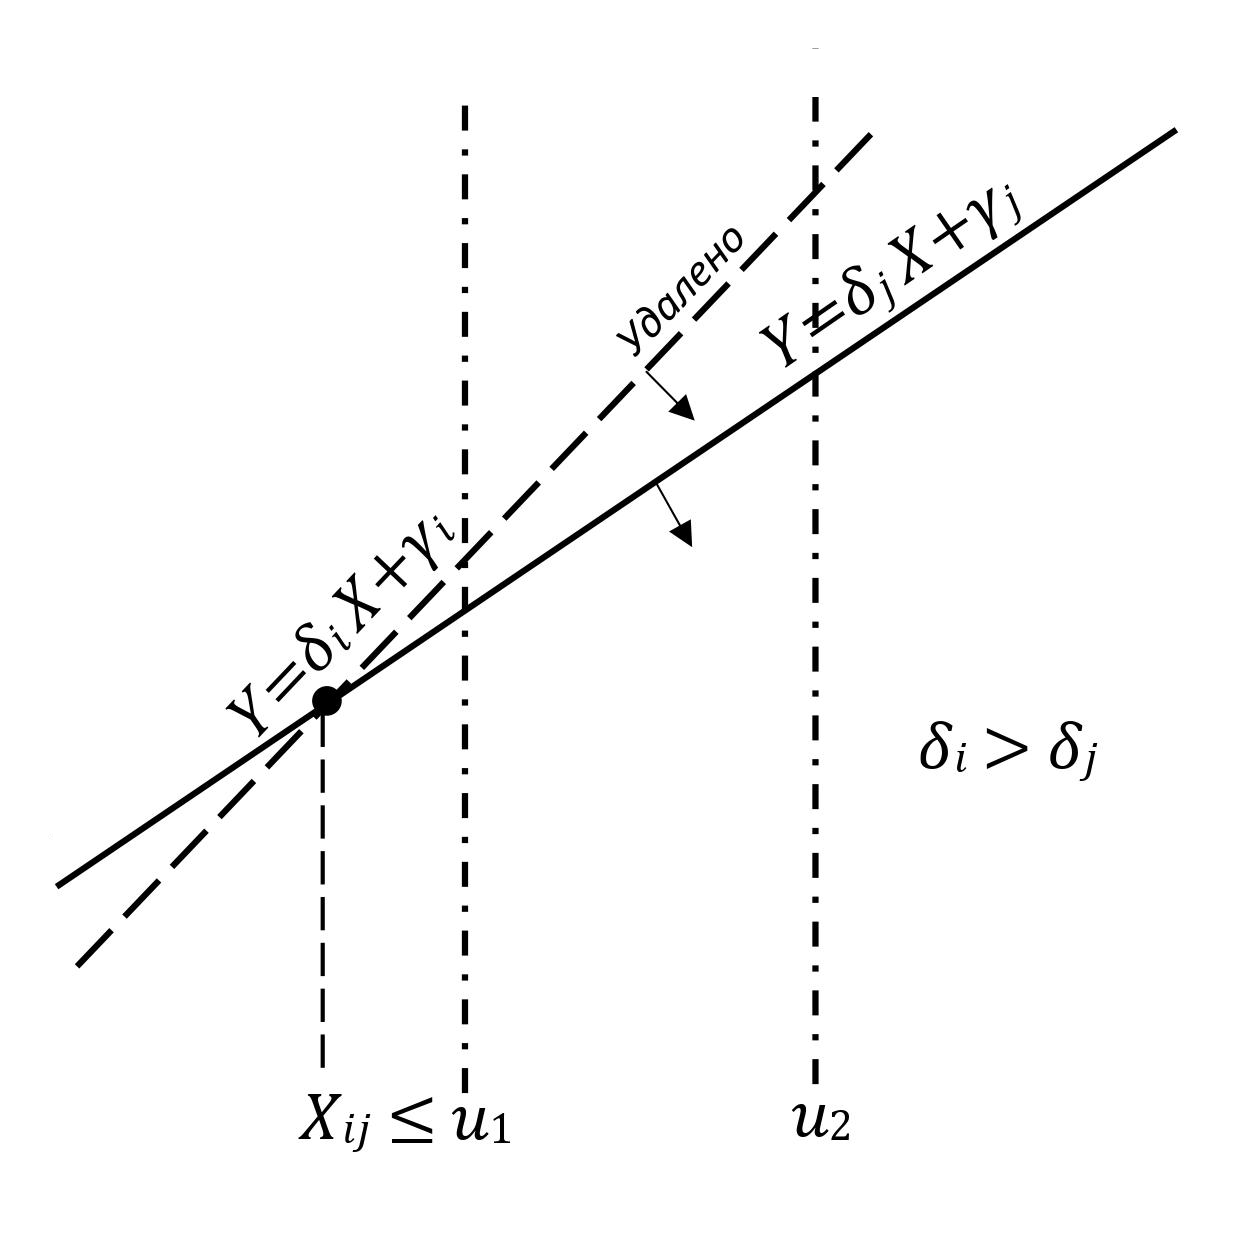
\includegraphics[width=1\linewidth]{Images/uu1} \\ a)}
\end{minipage}
\hfill
\begin{minipage}[h]{0.4\linewidth}
\center{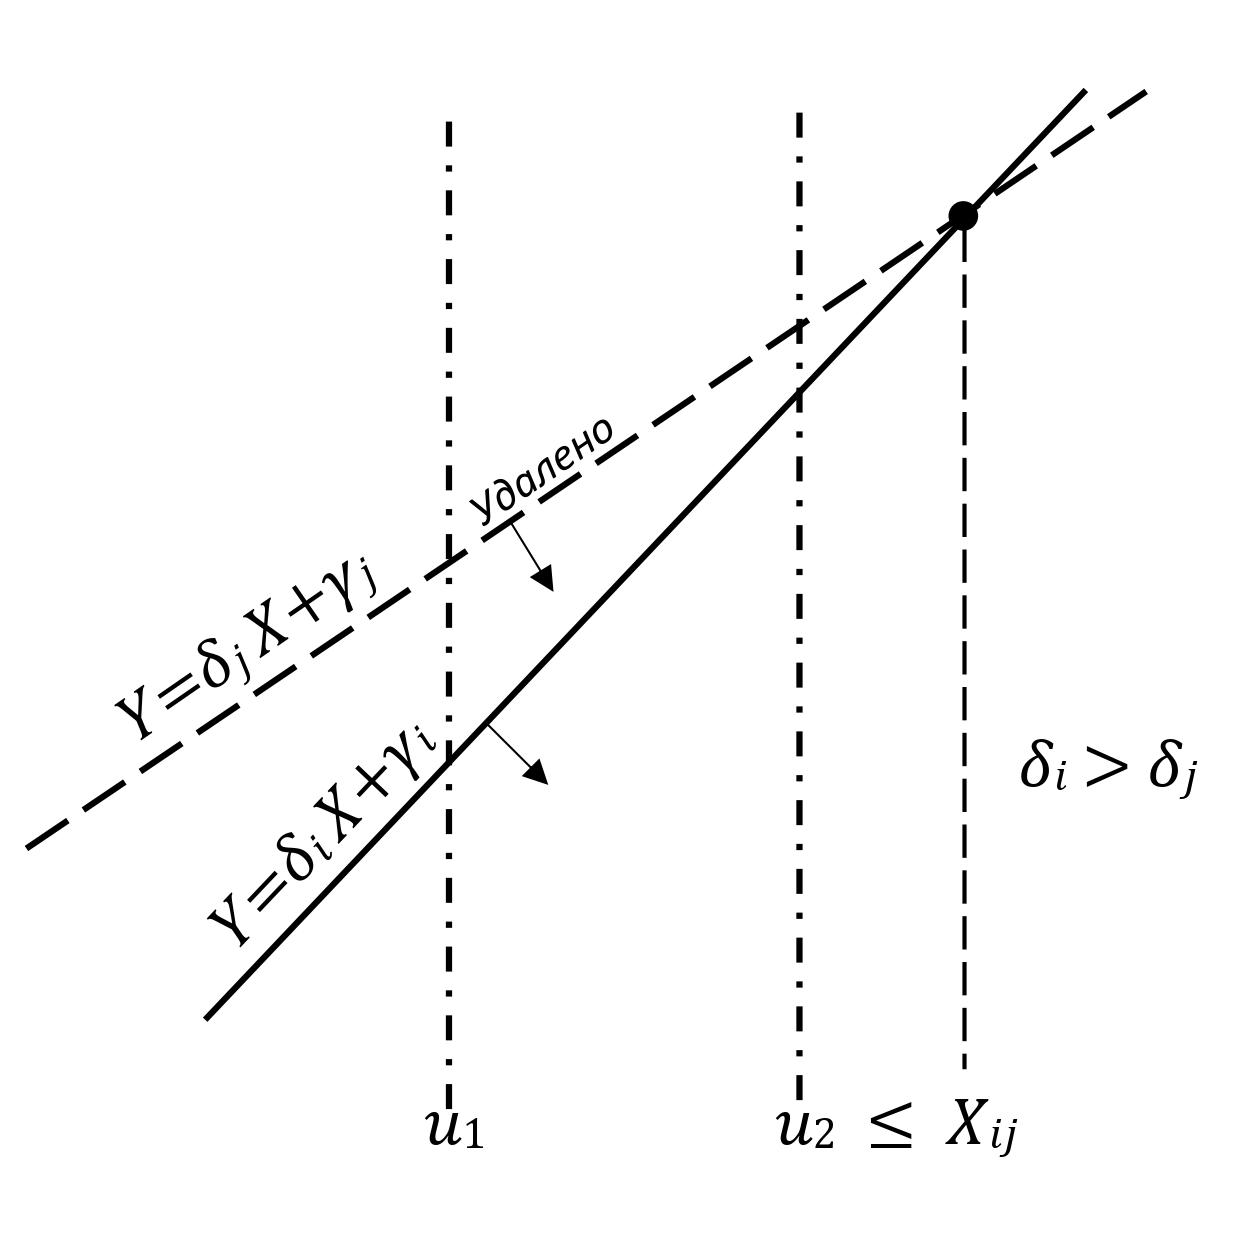
\includegraphics[width=1\linewidth]{Images/uu2} \\ b)}
\end{minipage}
\hfill
\begin{minipage}[h]{0.4\linewidth}
\center{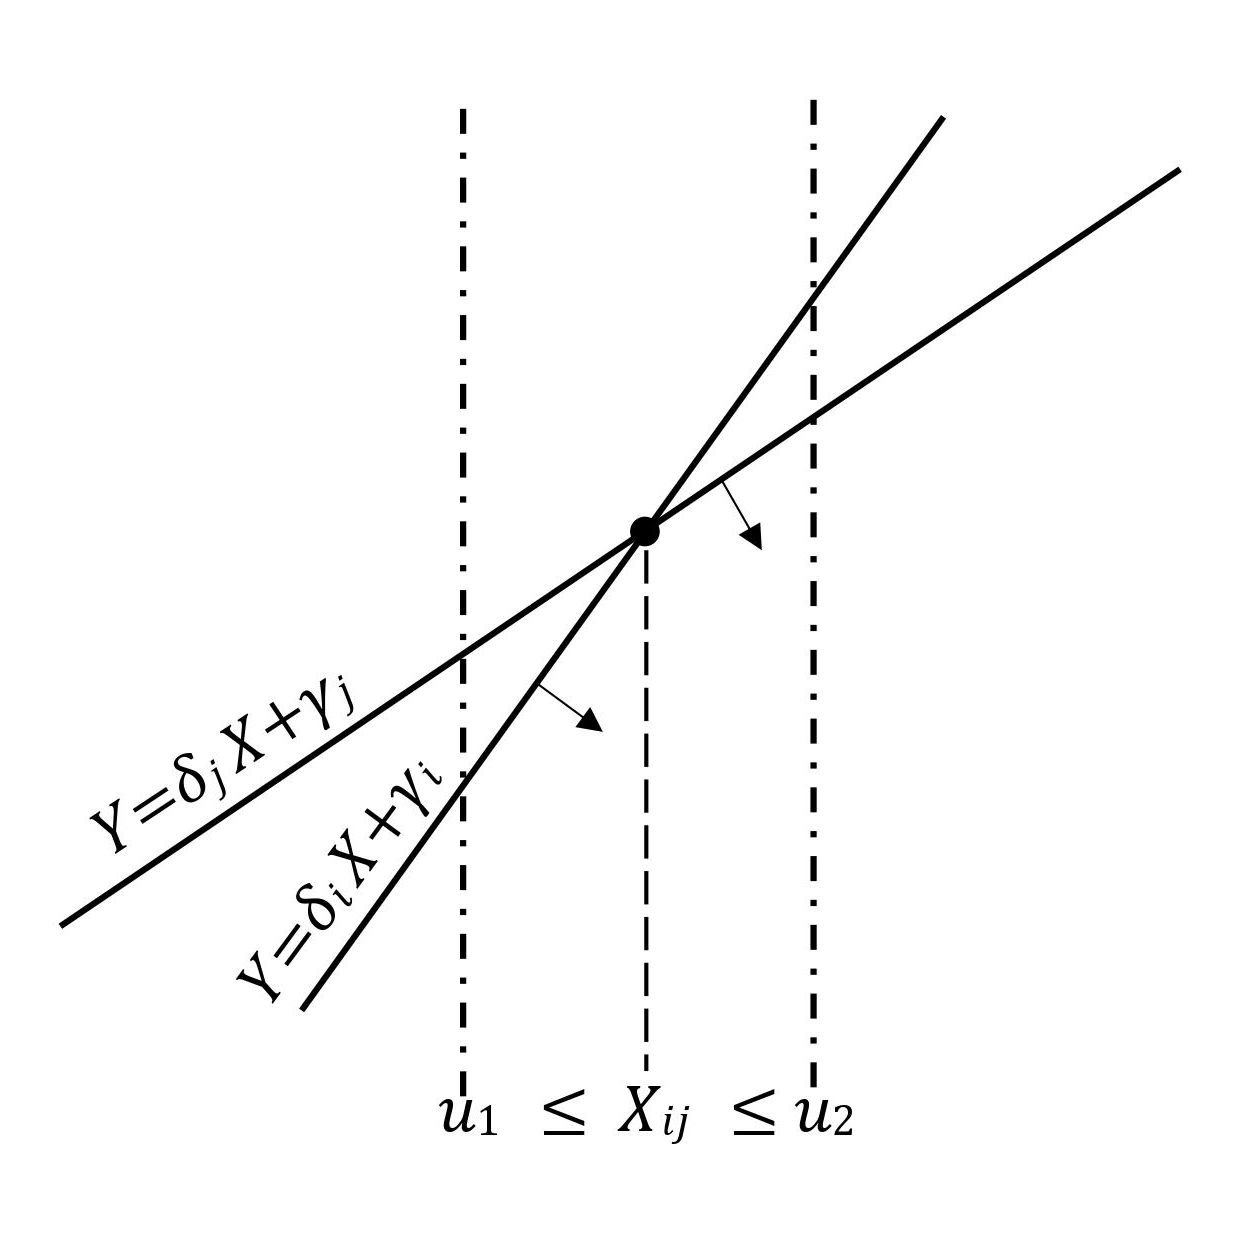
\includegraphics[width=1\linewidth]{Images/uu1u2} \\ c)}
\end{minipage}
\hfill
\begin{minipage}[h]{0.4\linewidth}
\center{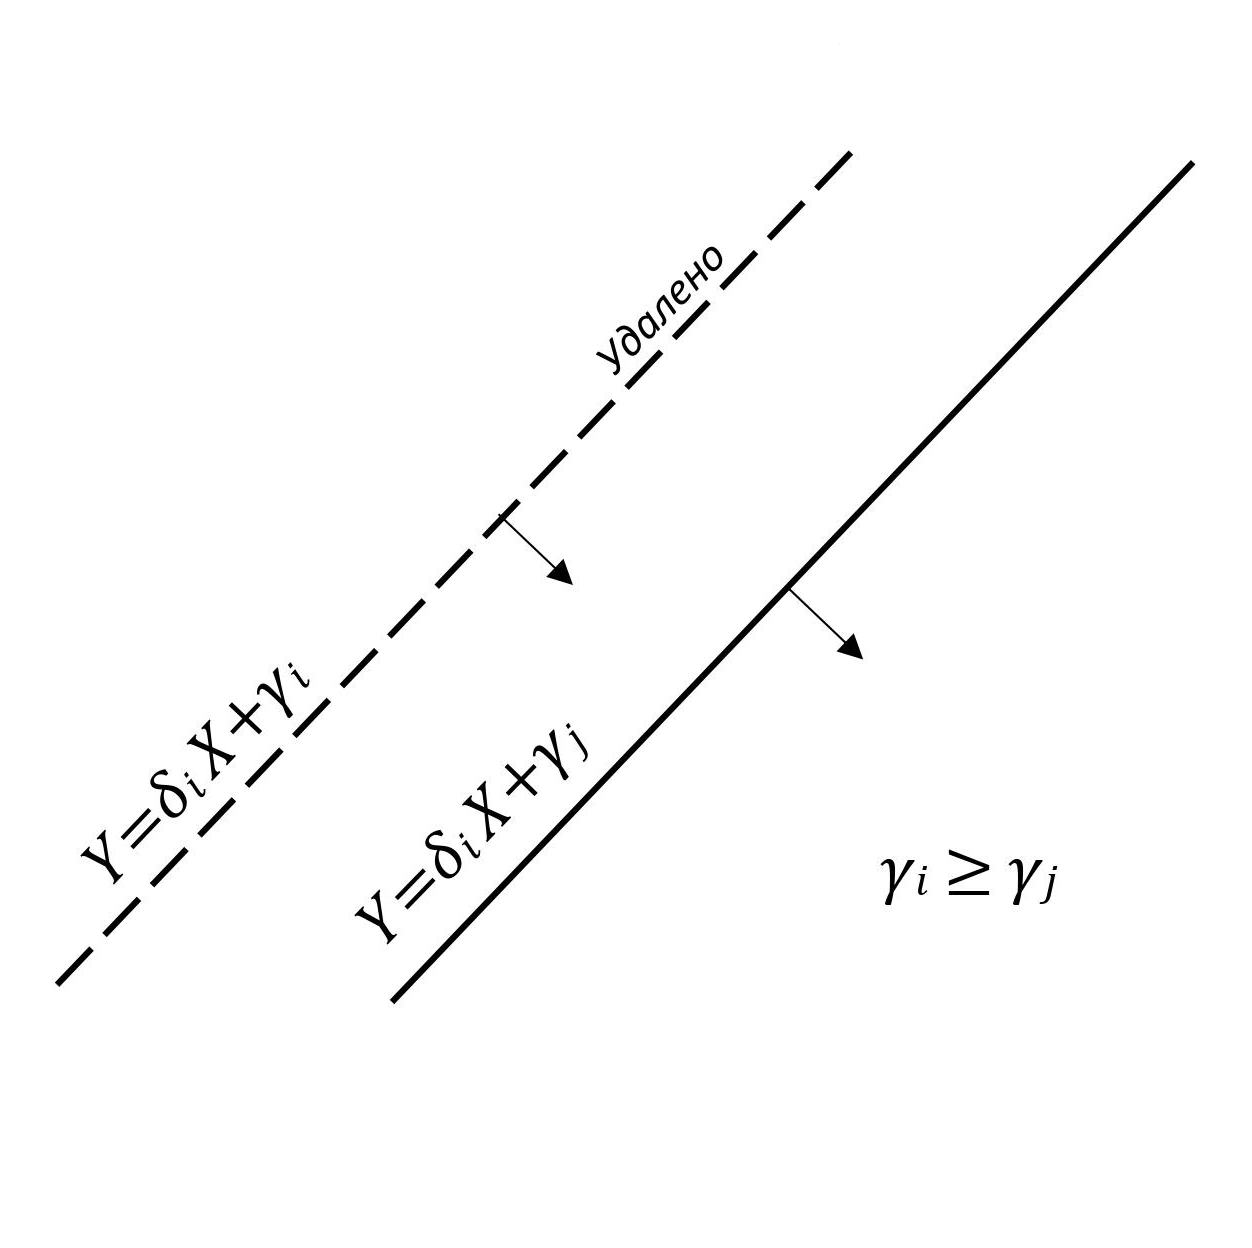
\includegraphics[width=1\linewidth]{Images/up} \\ d)}
\end{minipage}
\caption{$i,j \in I_{+}$.}
\label{ris:up}
\end{figure}
\end{enumerate}


%%%%%%%%%%%%%%%%%%%%%%%%%%%%%%%%%%%%%%%%%%%%%%%%%%%%%


\newpage
Для пар, из которых не было удалено ни одного ограничения, вычисляем абсциссу точки пересечения.\par
Если $k$ ограничений были удалены после первой итерации, то получаем множество из $\lfloor\frac{M-k}{2}\rfloor$ абсцисс точек пересечений, причём тратим на это $O(M)$ времени. Далее используя на этом множестве алгоритм нахождения медианы, обладающий линейной оценкой по времени \cite{Hopk00}, получаем медиану $\bar X$. 
Далее, проверяем наклоны и функции в абсциссе медианы, по вышеперечисленным правилам, и если в точке $\bar X$ нет экстремума, то половина вычисленных абсцисс ${X_{ij}}$ лежит в области, в которой минимум не достигается, это следует из описанных выше утверждений о допустимости $X'$.
Для каждого  $X_{ij}$ из этой области можно удалить одно ограничение из пары, используя следующие правила:
\begin{enumerate}
\item Если $H(X)=F_{-}(X)-F_{+}(X)>0$, то $X'$ - недопустимо:
\begin{enumerate}
\item Если $X_{ij}$ слева от  $\bar X$, а допустимые значения справа, то есть\par  $f_{-}^{(R)}(X')<f_{+}^{(R)}(X')$, тогда:
\begin{enumerate}
\item Если $i,j \in I_{-}$, то удаляем ограничение, у которого значение $\delta$ меньше.
\item Если $i,j \in I_{+}$, то удаляем ограничение, у которого значение $\delta$ больше.
\end{enumerate}
\item Если $X_{ij}$ справа от  $\bar X$, а допустимые значения слева, то есть\par $f_{-}^{(L)}(X')>f_{+}^{(L)}(X')$, тогда:
\begin{enumerate} 
\item Если $i,j \in I_{-}$, то удаляем ограничение, у которого значение $\delta$ больше.
\item Если $i,j \in I_{+}$, то удаляем ограничение, у которого значение $\delta$ меньше.
\end{enumerate}
\end{enumerate}
\item Если $H(X)=F_{-}(X)-F_{+}(X)\leqslant 0$, то $X'$ - допустимо:
\begin{enumerate}
\item Если $X_{ij}$ слева от  $\bar X$, а оптимум - справа, то есть\par  $f_{-}^{(L)}(\bar X)\leqslant f_{-}^{(R)}(\bar X)<0$, тогда:
\begin{enumerate}
\item Если $i,j \in I_{-}$, то удаляем ограничение, у которого значение $\delta$ меньше.
\item Если $i,j \in I_{+}$, то удаляем ограничение, у которого значение $\delta$ больше.
\end{enumerate}
\item Если $X_{ij}$ справа от  $\bar X$, а оптимум - слева, то есть\par $f_{-}^{(R)}(\bar X)\geqslant f_{-}^{(L)}(\bar X)>0$, тогда:
\begin{enumerate} 
\item Если $i,j \in I_{-}$, то удаляем ограничение, у которого значение $\delta$ больше.
\item Если $i,j \in I_{+}$, то удаляем ограничение, у которого значение $\delta$ меньше.
\end{enumerate}
\end{enumerate}
\end{enumerate}
Завершаем шаг алгоритма с результатом, что удалено не менее $k+\lceil \frac {\lfloor\frac{M-k}{2}\rfloor}{2}\rceil \geqslant \lfloor\frac{M}{4}\rfloor$ ограничений. Это является подтверждением того, что $\alpha = \frac{1}{4}$ и получаем следующий результат в виде теоремы: \par
\begin{theorem}
Задачу линейного программирования с двумя переменными и $N$ ограничениями можно решить за оптимальное время $O(N)$. 
\end{theorem}


%%%%%%%%%%%%%%%%%%%%%%%%%%%%%%%%%%%%%%%%%%%%%%%

\newpage
\section{Алгоритм выбора k-й порядковой статистики.}
В алгоритме Мегиддо для выбора медианы используется алгоритм выбора  k-й порядковой статистики, который имеет линейную временную оценку.\cite{Hopk00}\par
Алгоритм состоит в следующем:\par
\begin{enumerate}
\item Пока  $n\geqslant 75$:\par
\begin{enumerate}
\item Разделяем n элементов на группы по 5 элементов, не беря во внимание группу из 1-4 элементов, не вошедших в другие группы. 
\item Сортируем каждую группу любым алгоритмов и берём средние элементы из каждой группы. Всего таких средних элементов будет [$\frac{n}{5}$]. (Рис.~\ref{ris:m5})
\end{enumerate}
\item Когда $n$ станет меньше или равно 75, то:\par
Сортируем и выбираем элемент стоящий по середине, это и будет медиана, если количество элементов на последнем шаге чётное, то из двух берём то число,которое ближе к среднему значению между всеми элементами. 
\end{enumerate}

\begin{figure}[h]
\center{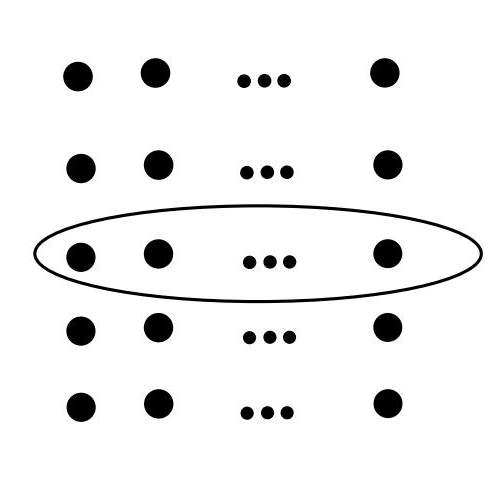
\includegraphics[width=0.3\linewidth]{Images/m5}}
\caption{Иллюстрация работы шага алгоритма.}
\label{ris:m5}
\end{figure}


%%%%%%%%%%%%%%%%%%%%%%%%%%%%%%%%%%

\newpage
\section{Вычислительные эксперименты.}
Чтобы проверить работу алгоритмов, реализованных в ходе выполнения дипломной работы, были проведены следующие эксперименты для практического доказательства теоритических оценок эффективности.\par
Для реализованного мной алгоритма поиска медианы было произведено сравнение с алгоримом стандартной быстрой сортировки, из библиотеки <stdlib.h>, с последующим взятием среднего значения. На вход подавались массивы содержащие значения типа double сгенерированные с помощью функции rand(), из библиотеки <stdlib.h>. На выходе выдавалось значение медианы, которое для совпадало для обоих алгоритмов, что является гарантом правильности работы моего линейного алгоритма поиска медианы, а так же время работы и ускорение, которое может быть получено, если использовать мой алгоритм. Результаты представлены в таблице (Таб.~\ref{tab:Med}) и на графиках.(Рис.~\ref{ris:0001}, Рис.~\ref{ris:0002}, Рис.~\ref{ris:0003}, Рис.~\ref{ris:0004})

\begin{table}[h!]
\caption{\label{tab:Med}Работа алгоритма линейного поиска медианы и алгоритма быстрой сортировки.}
\begin{center}
\begin{tabular}{|c|c|c|c|}
\hline
Размер массива & Лин.поиск медианы, мс  & Быстр. сорт. & Ускор.\\
\hline
1000000 & 4 & 195 & 48.75    \\
\hline
10000000& 41& 1740 & 42.4    \\
\hline
20000000 & 91 & 3467 & 38    \\
\hline
30000000 & 123 & 5162 & 41.9   \\
\hline
40000000 & 164 & 6867 & 41.8   \\
\hline
50000000 & 195 & 8623 & 44.2  \\
\hline
60000000 & 239 & 10319 & 43.17   \\
\hline
70000000 & 316 & 12012 & 36.3   \\
\hline
80000000 & 350 & 13675 & 43.2 \\
\hline
90000000 & 400 & 15834 & 43.3   \\
\hline
100000000 & 521 & 17904 & 34.4  \\
\hline
\end{tabular}
\end{center}
\end{table} 

%%%%%%%%%%%%%%%%

\newpage
\begin{figure}[h!]
\center{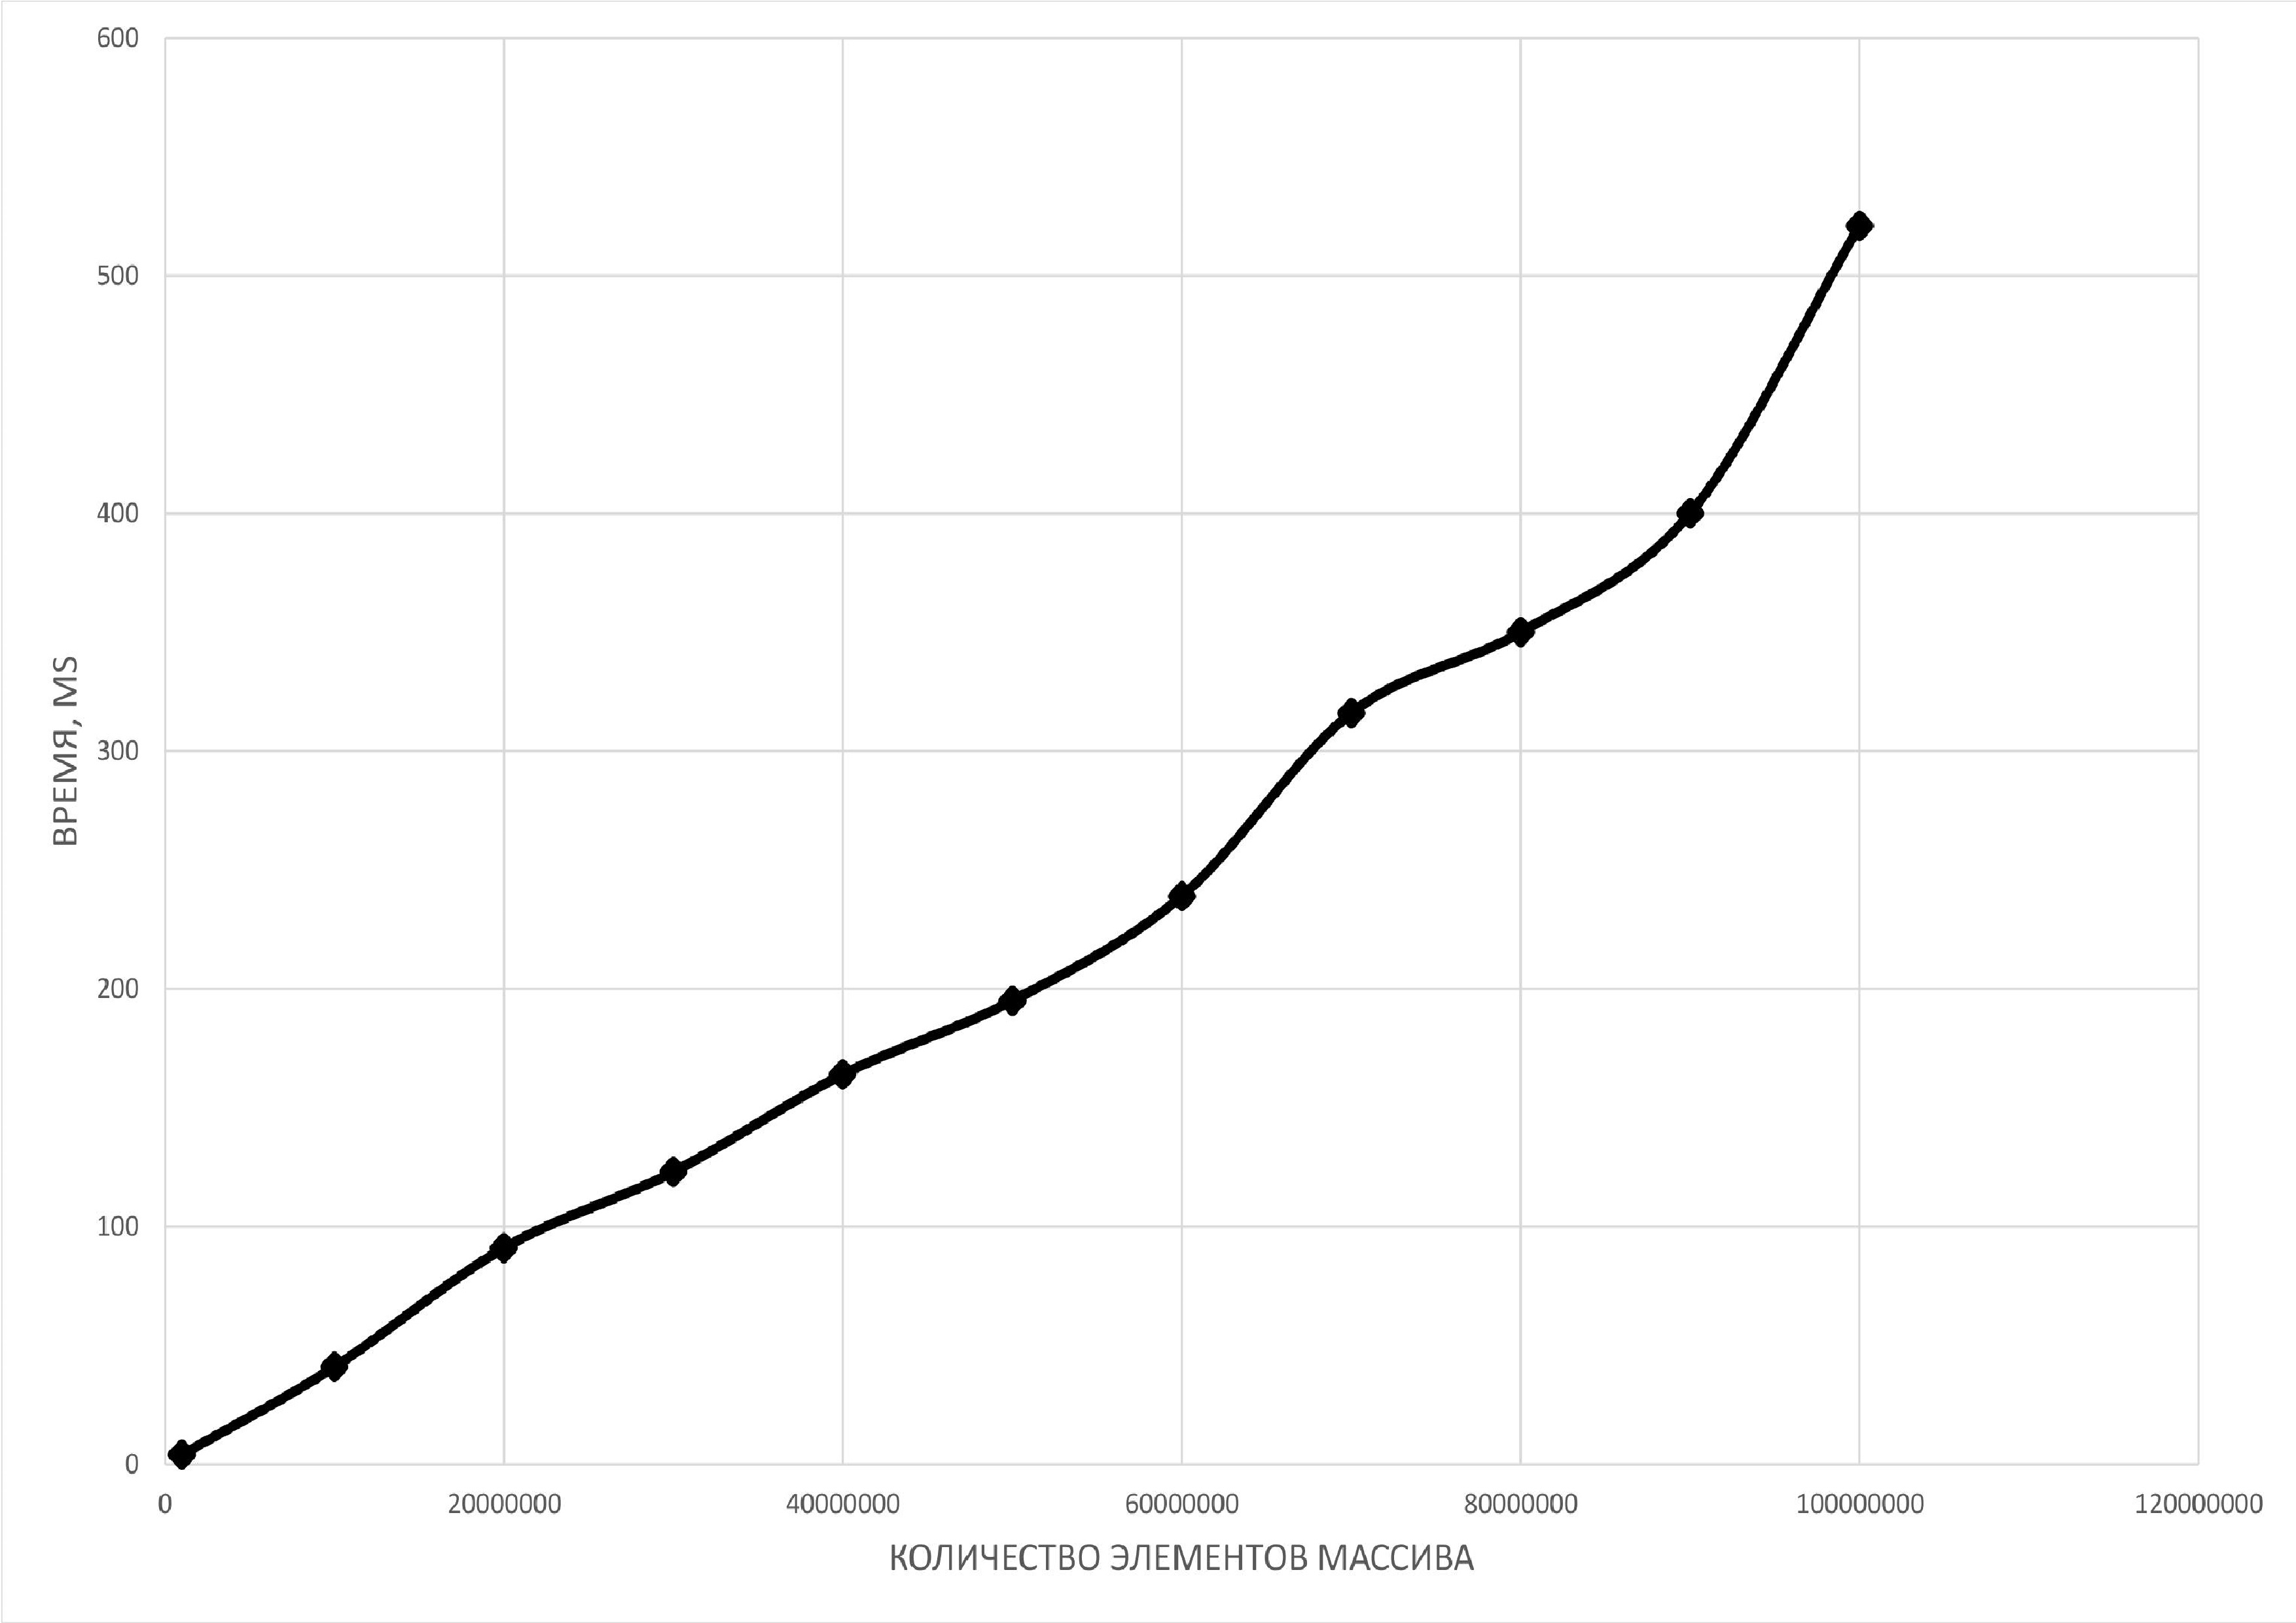
\includegraphics[width=0.9\linewidth]{Images/00011}}
\caption{Работа линейного алгоритма поиска медианы.}
\label{ris:0001}
\end{figure}


\begin{figure}[h!]
\center{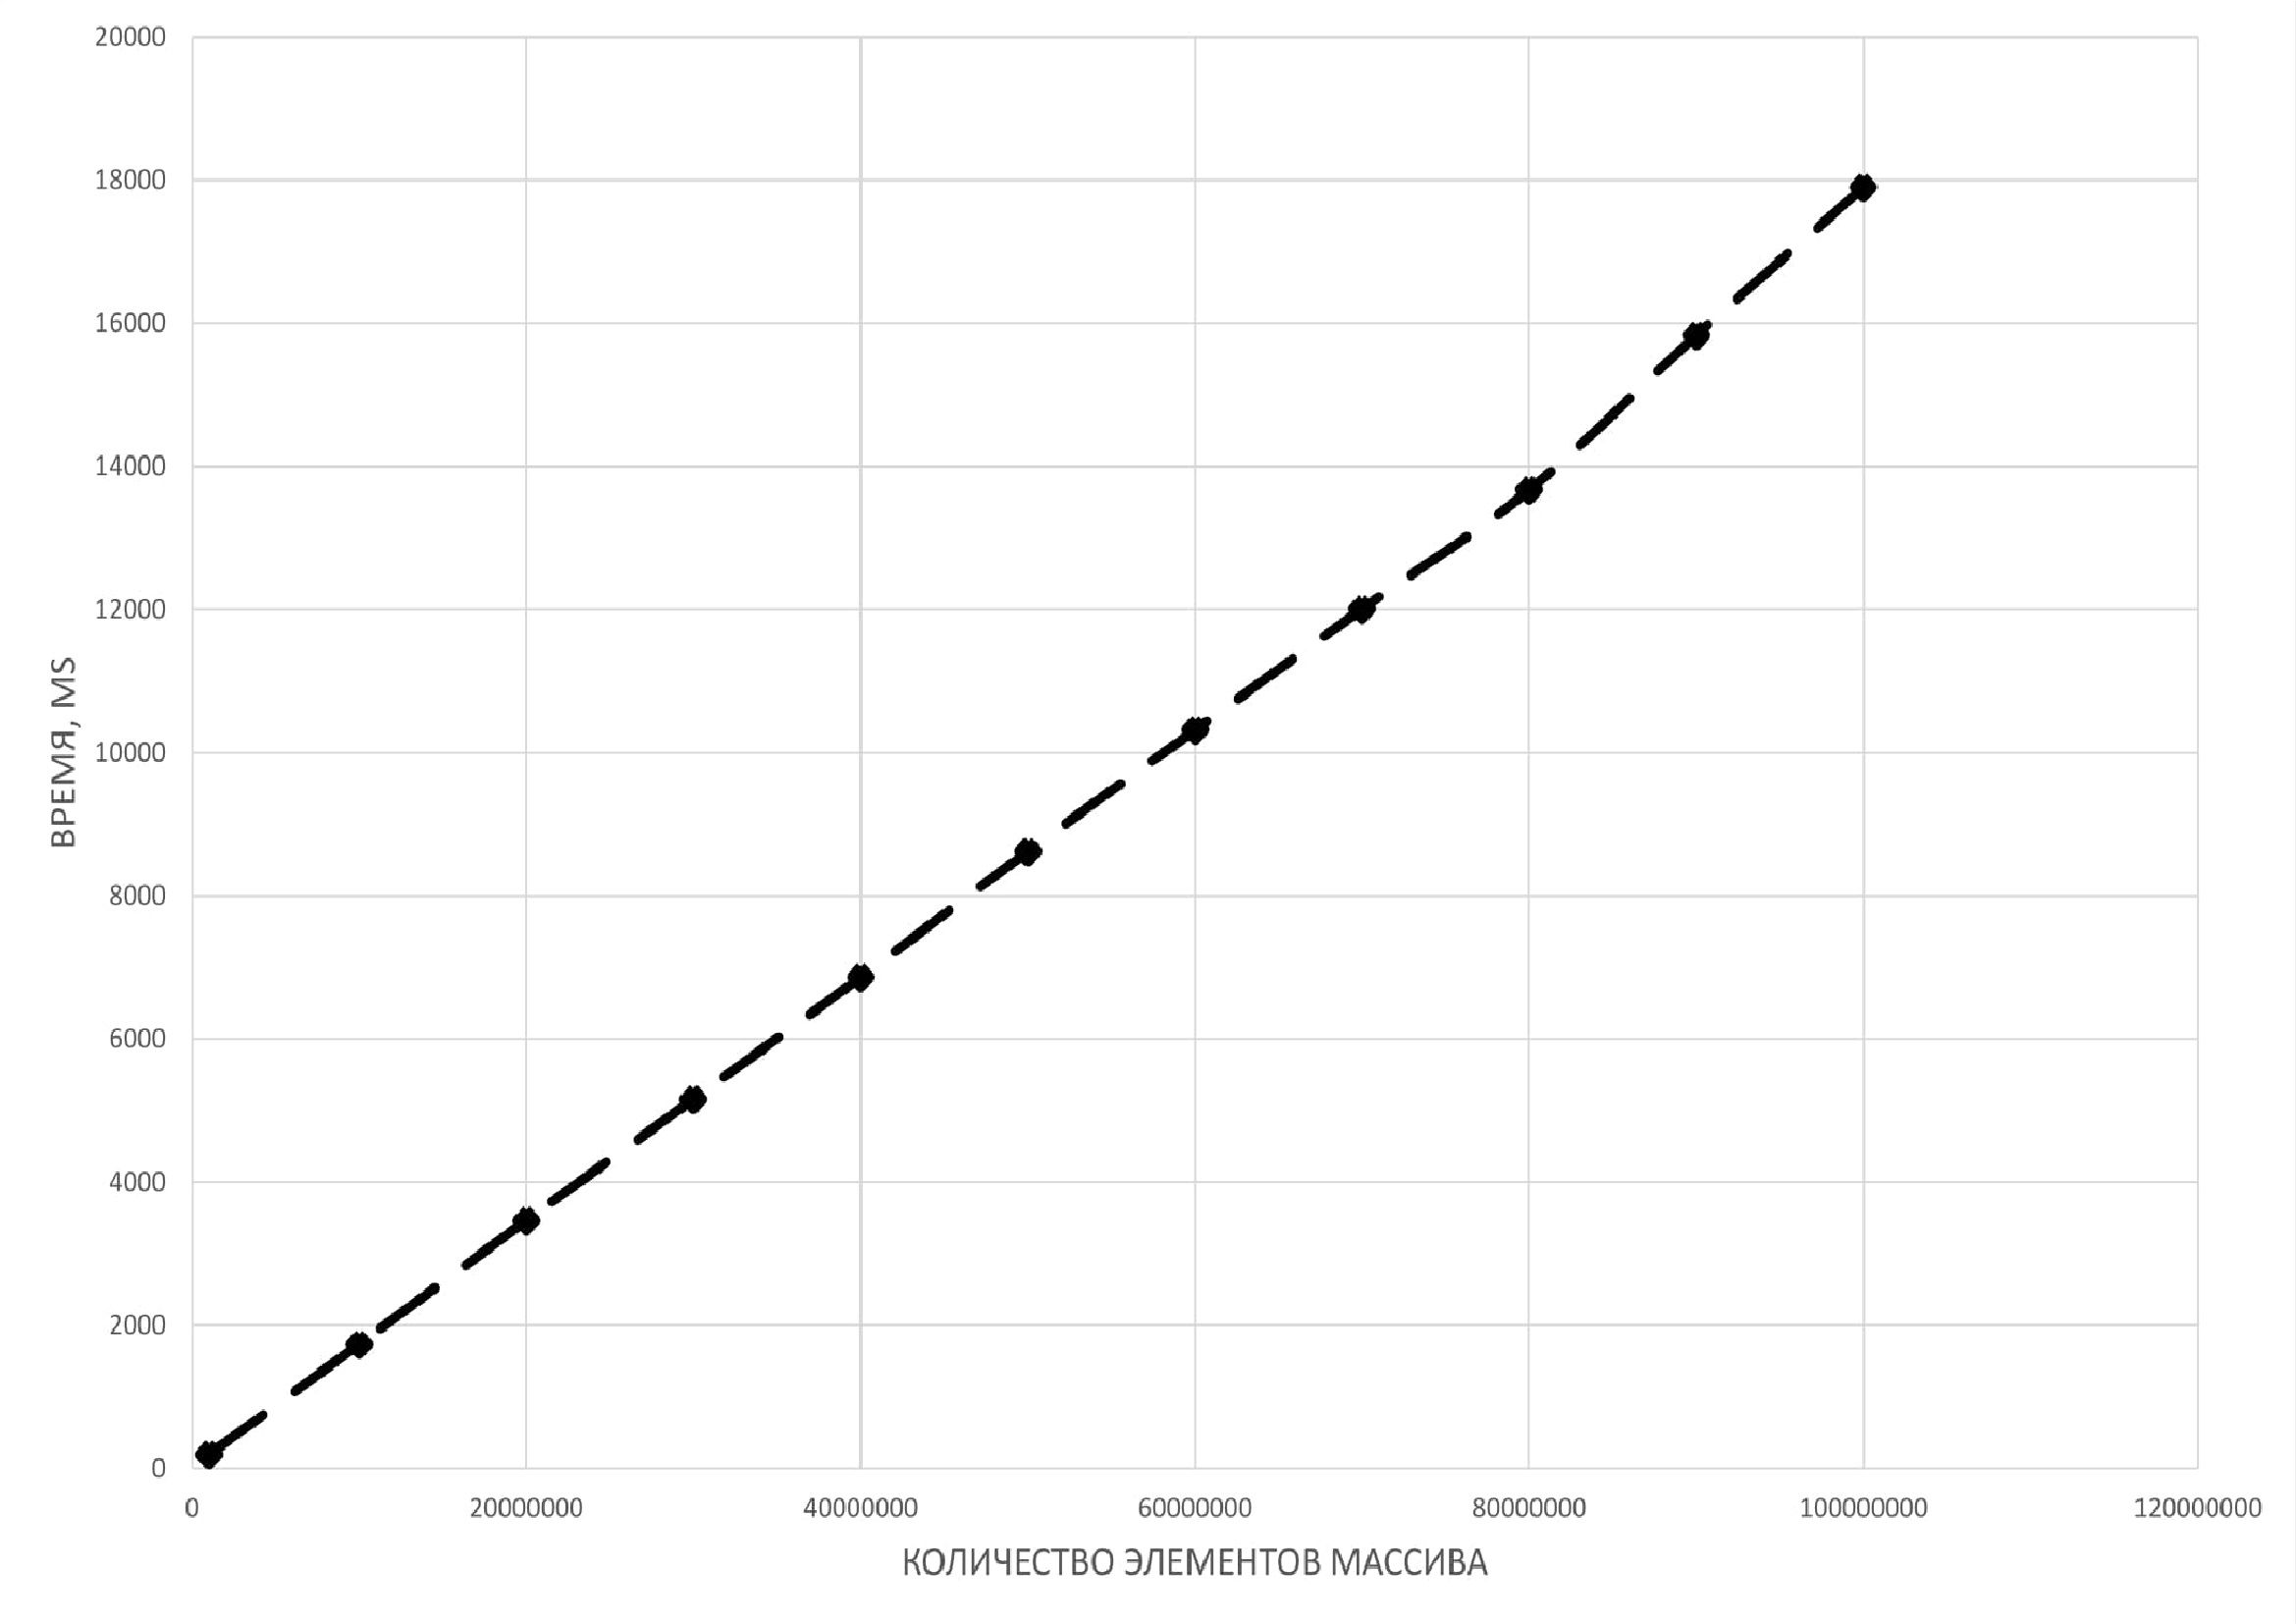
\includegraphics[width=0.9\linewidth]{Images/00021}}
\caption{Работа алгоритма быстрой сортировки.}
\label{ris:0002}
\end{figure}

\newpage
\begin{figure}[h!]
\center{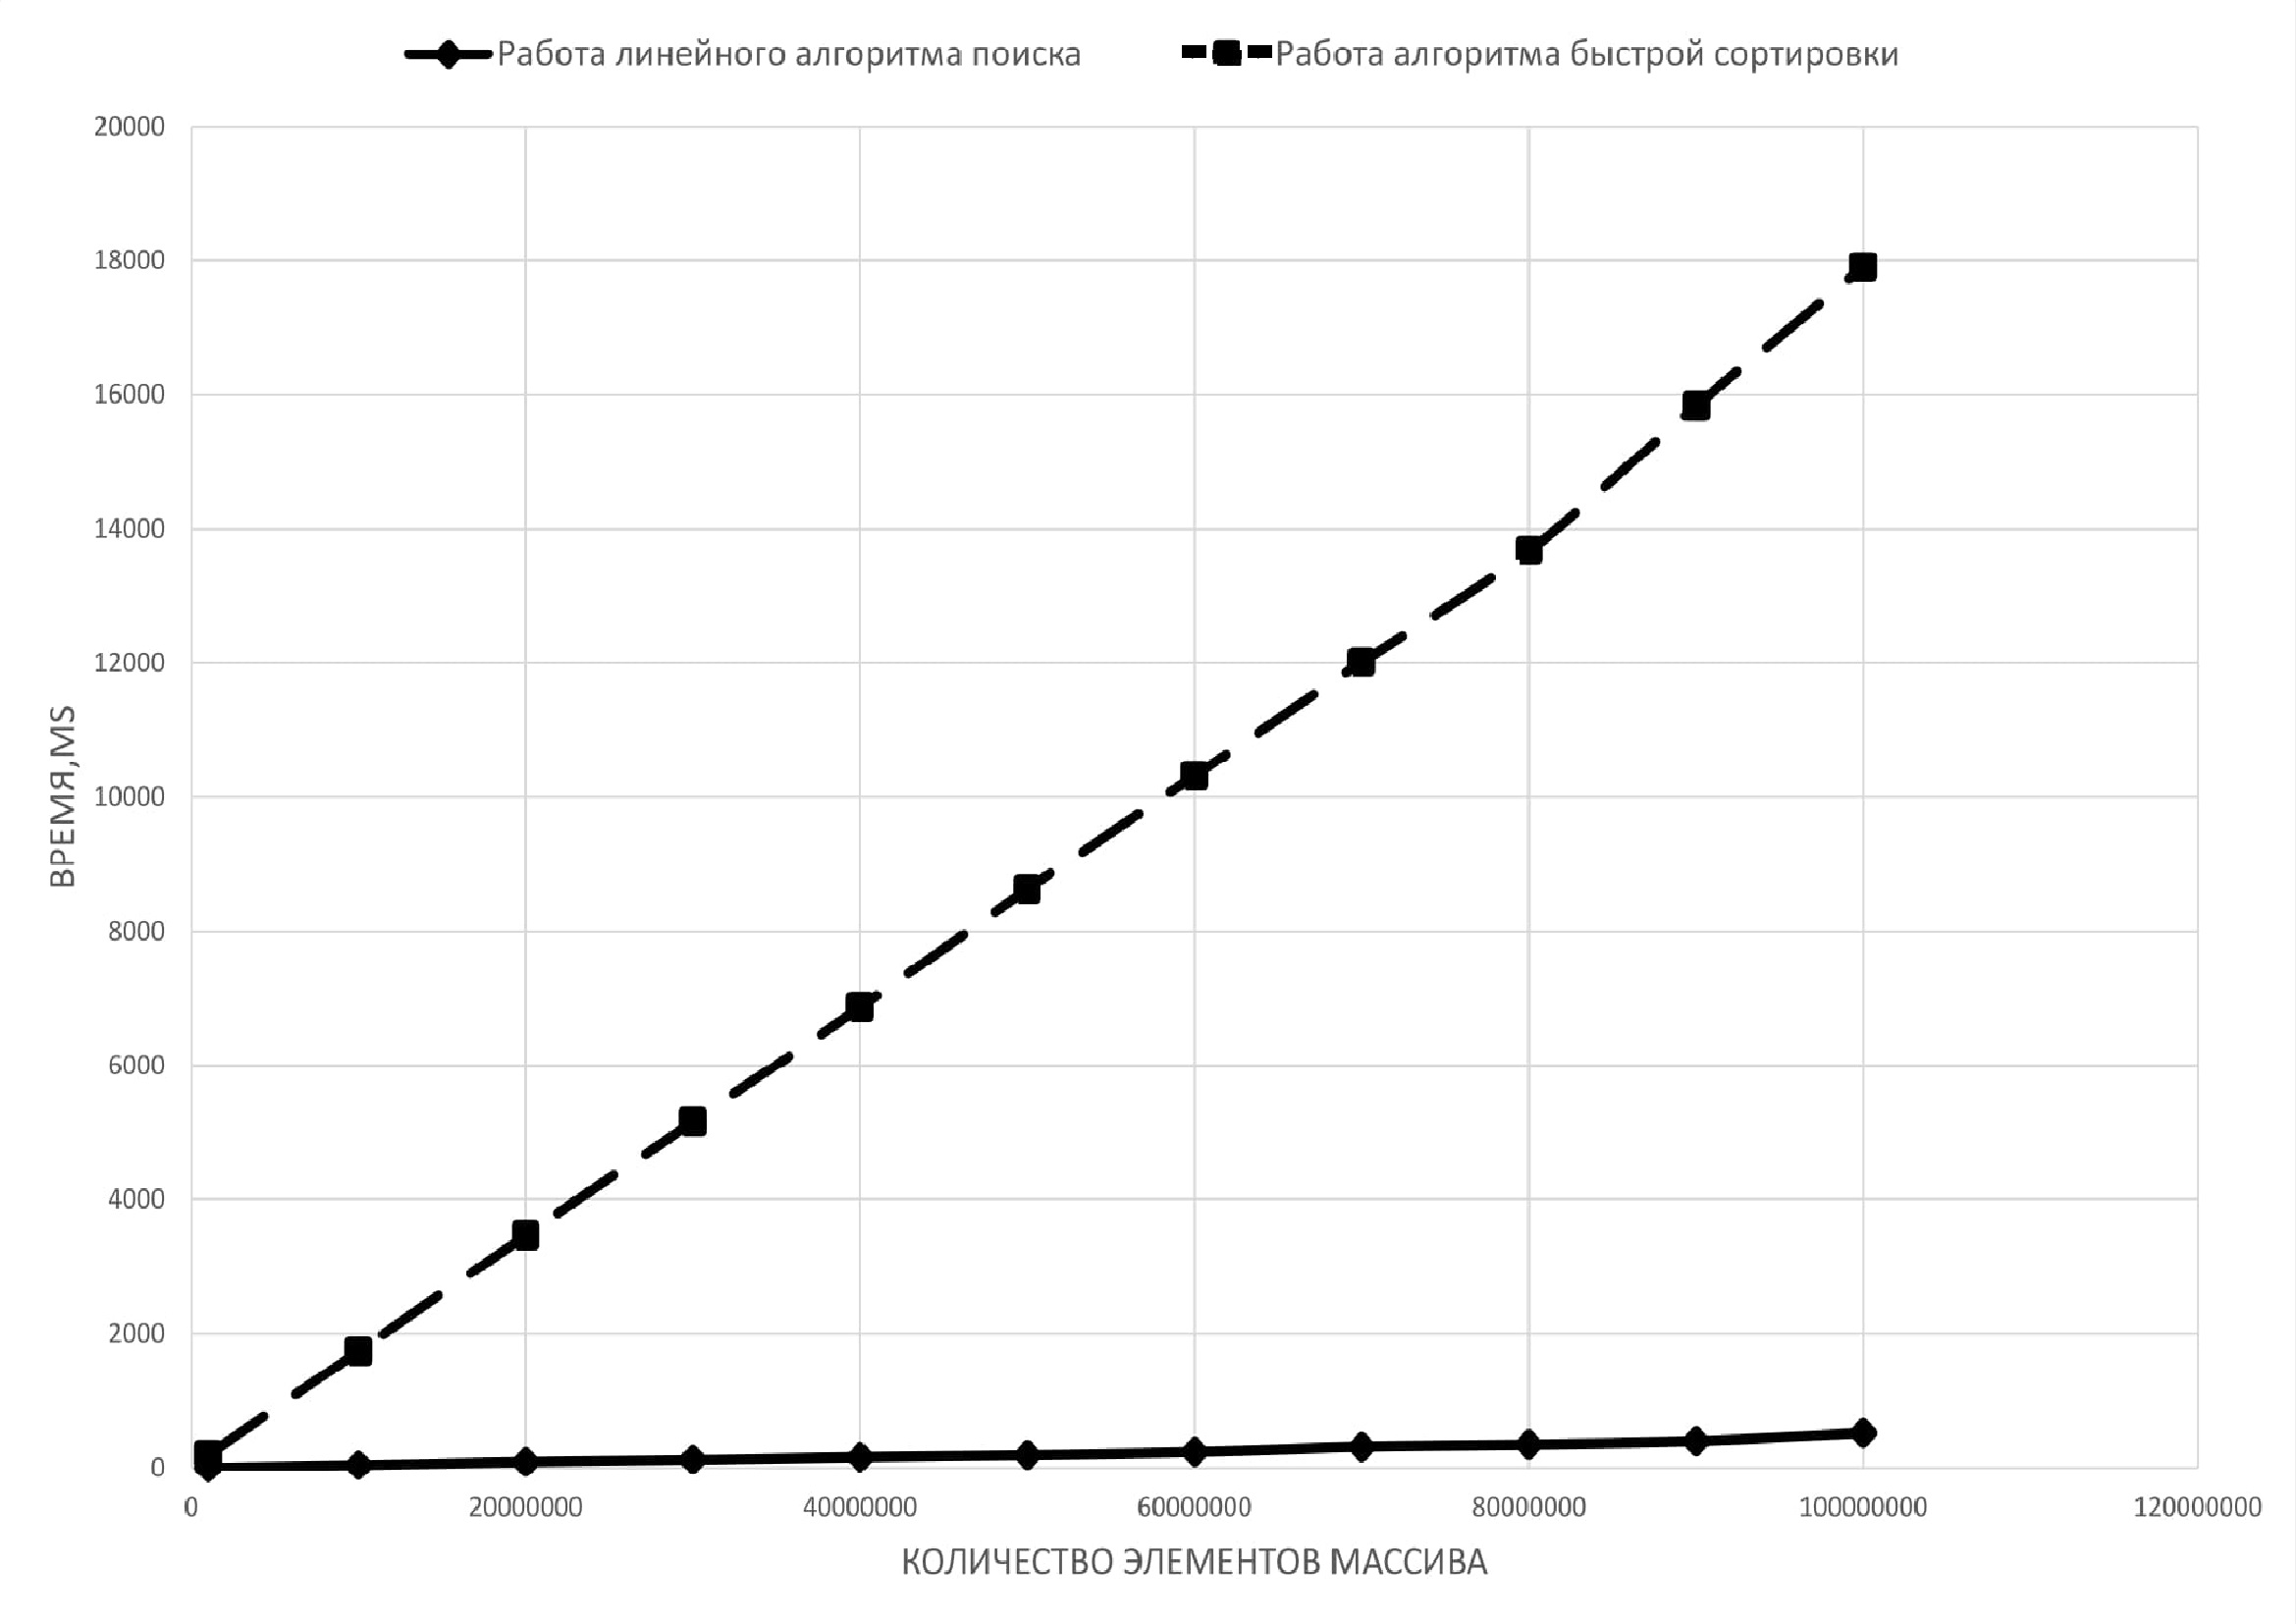
\includegraphics[width=0.9\linewidth]{Images/00031}}
\caption{Сравнение работы алгоритмов.}
\label{ris:0003}
\end{figure}


\begin{figure}[h!]
\center{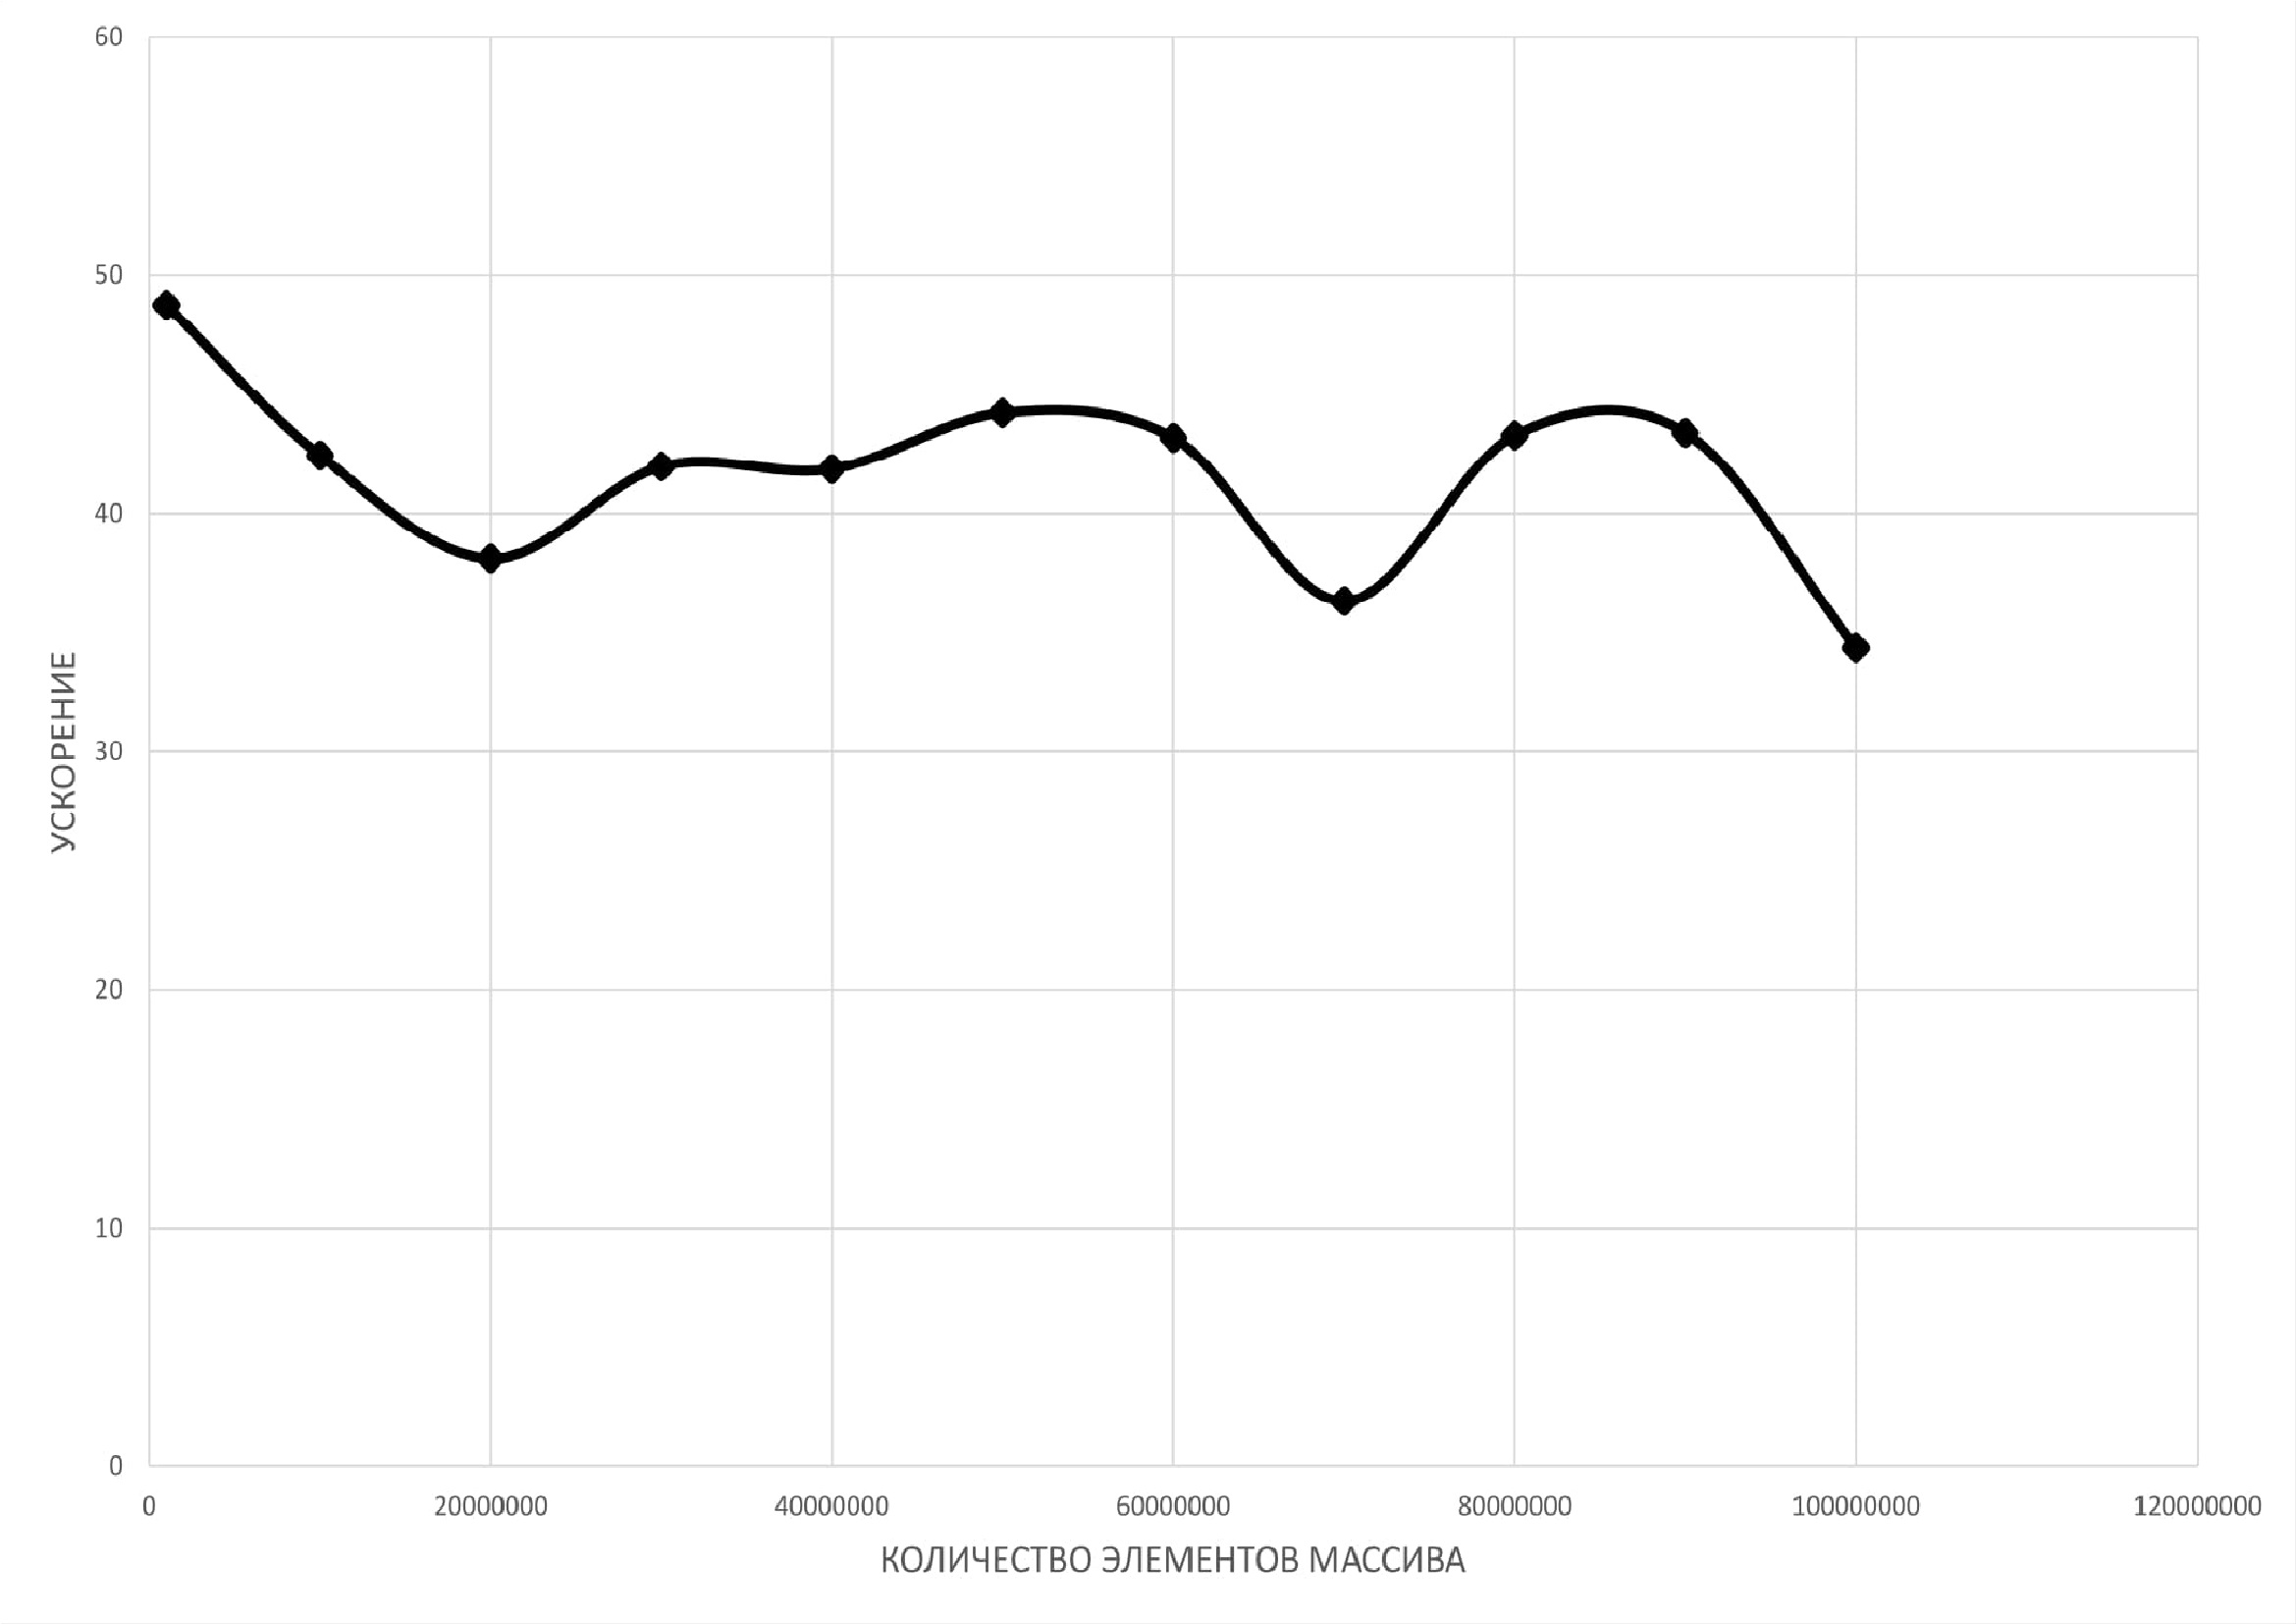
\includegraphics[width=0.9\linewidth]{Images/00041}}
\caption{Ускорение.}
\label{ris:0004}
\end{figure}

%%%%%%%%%%%%%%%%%%%%%%%%%%%%%%%


\newpage
Для реализованного мной оптимального алгоритма, решения задачи линейного программирования, были произведены эксперименты, результаты которых содержатся в таблице (Таб.~\ref{tab:Meg}) и графиках (Рис.~\ref{ris:Meg},  Рис.~\ref{ris:Meg2}). Исходя из результатов экспериментов можно получить оценку алгоритма Меггидо для класса задач, на котором производились экспериметы. Эта оценка равна $15.25m$, где m - количество ограничений. 


\begin{table}[h!]
\caption{\label{tab:Meg}Работа алгоритма Мегиддо.}
\begin{center}
\begin{tabular}{|c|c|c|}
\hline
Кол-во ограничений & Среднее время, мс  & Среднее число итераций\\%Эксп 1& Эксп 2& Эксп 3\\
\hline
1000 & 2.2 & 15960 \\%2 & 3 & 2   \\
\hline
10000 & 3.8 & 146192\\ %4 & 4 & 4   \\
\hline
100000 & 17.2 & 1549131\\%18 & 17 & 16   \\
\hline
1000000 & 178.2 & 16051588\\% 176 & 164 & 171  \\
\hline
2500000 & 446 & 39341976\\% 430 & 460 & 434  \\
\hline
5000000 & 836.8 & 75951167\\%787 & 877 & 825  \\
\hline
7500000 & 1296.4 & 114465857\\%1267 & 1304 & 1278  \\
\hline
10000000 & 1682.4 & 152503343\\%1623 & 1663 & 1691  \\
\hline
12500000 & 2055.2 & 189718547\\%1997 & 2009 & 2035  \\
\hline
15000000 & 2435.6 & 227678646\\%2360 & 2375 & 2441  \\
\hline
17500000 & 2752.2 & 265569980\\% 2734 & 2773 & 2786  \\
\hline
20000000 & 3116.2 & 286668923\\%3220 & 3110 & 3140  \\
\hline
22500000 & 3583.6 & 338076038\\%3601 & 3545 & 3653   \\
\hline
25000000 & 3876.4 & 379477170\\%3839 & 3905 & 3851   \\
\hline
27500000 & 4314.2 & 417948983\\%4234 & 4315 & 4391   \\
\hline
30000000 & 4537.8 & 456232002\\%4531 & 4555 & 4539   \\
\hline
\end{tabular}
\end{center}
\end{table} 

\newpage
\begin{figure}[h!]
\center{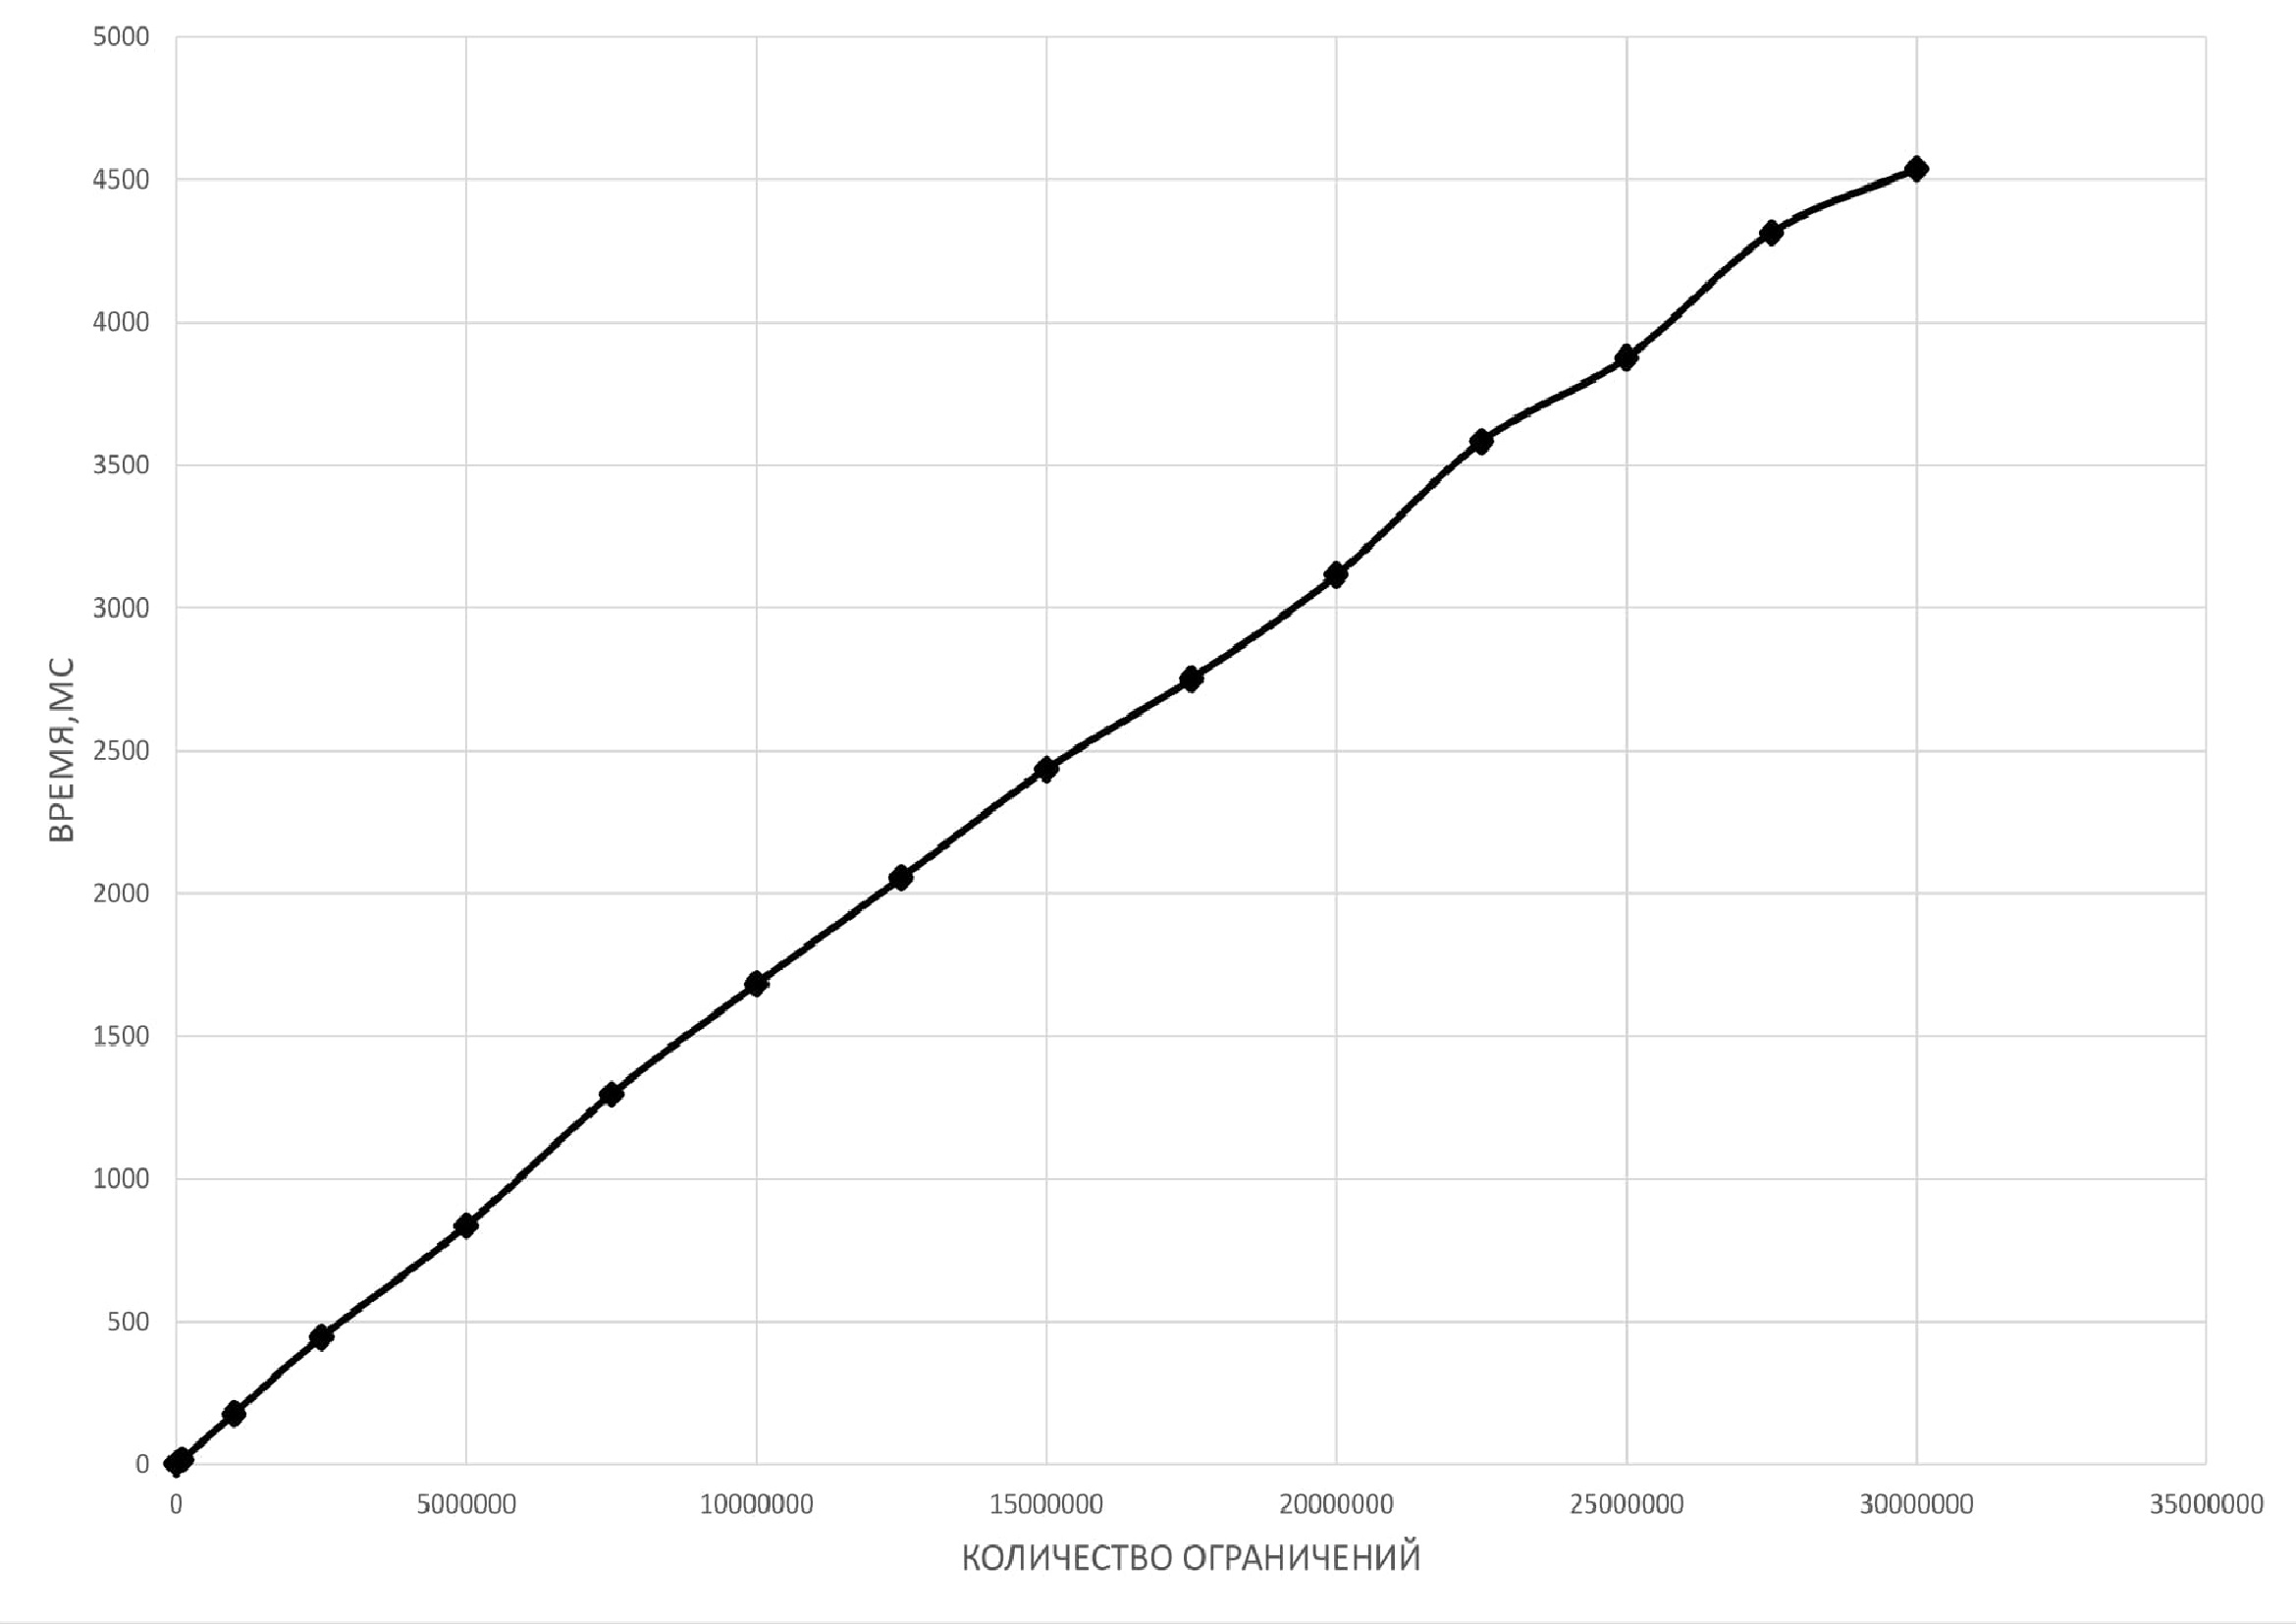
\includegraphics[width=0.9\linewidth]{Images/Megiddo}}
\caption{Работа алгоритма Мегиддо.}
\label{ris:Meg}
\end{figure}


\begin{figure}[h!]
\center{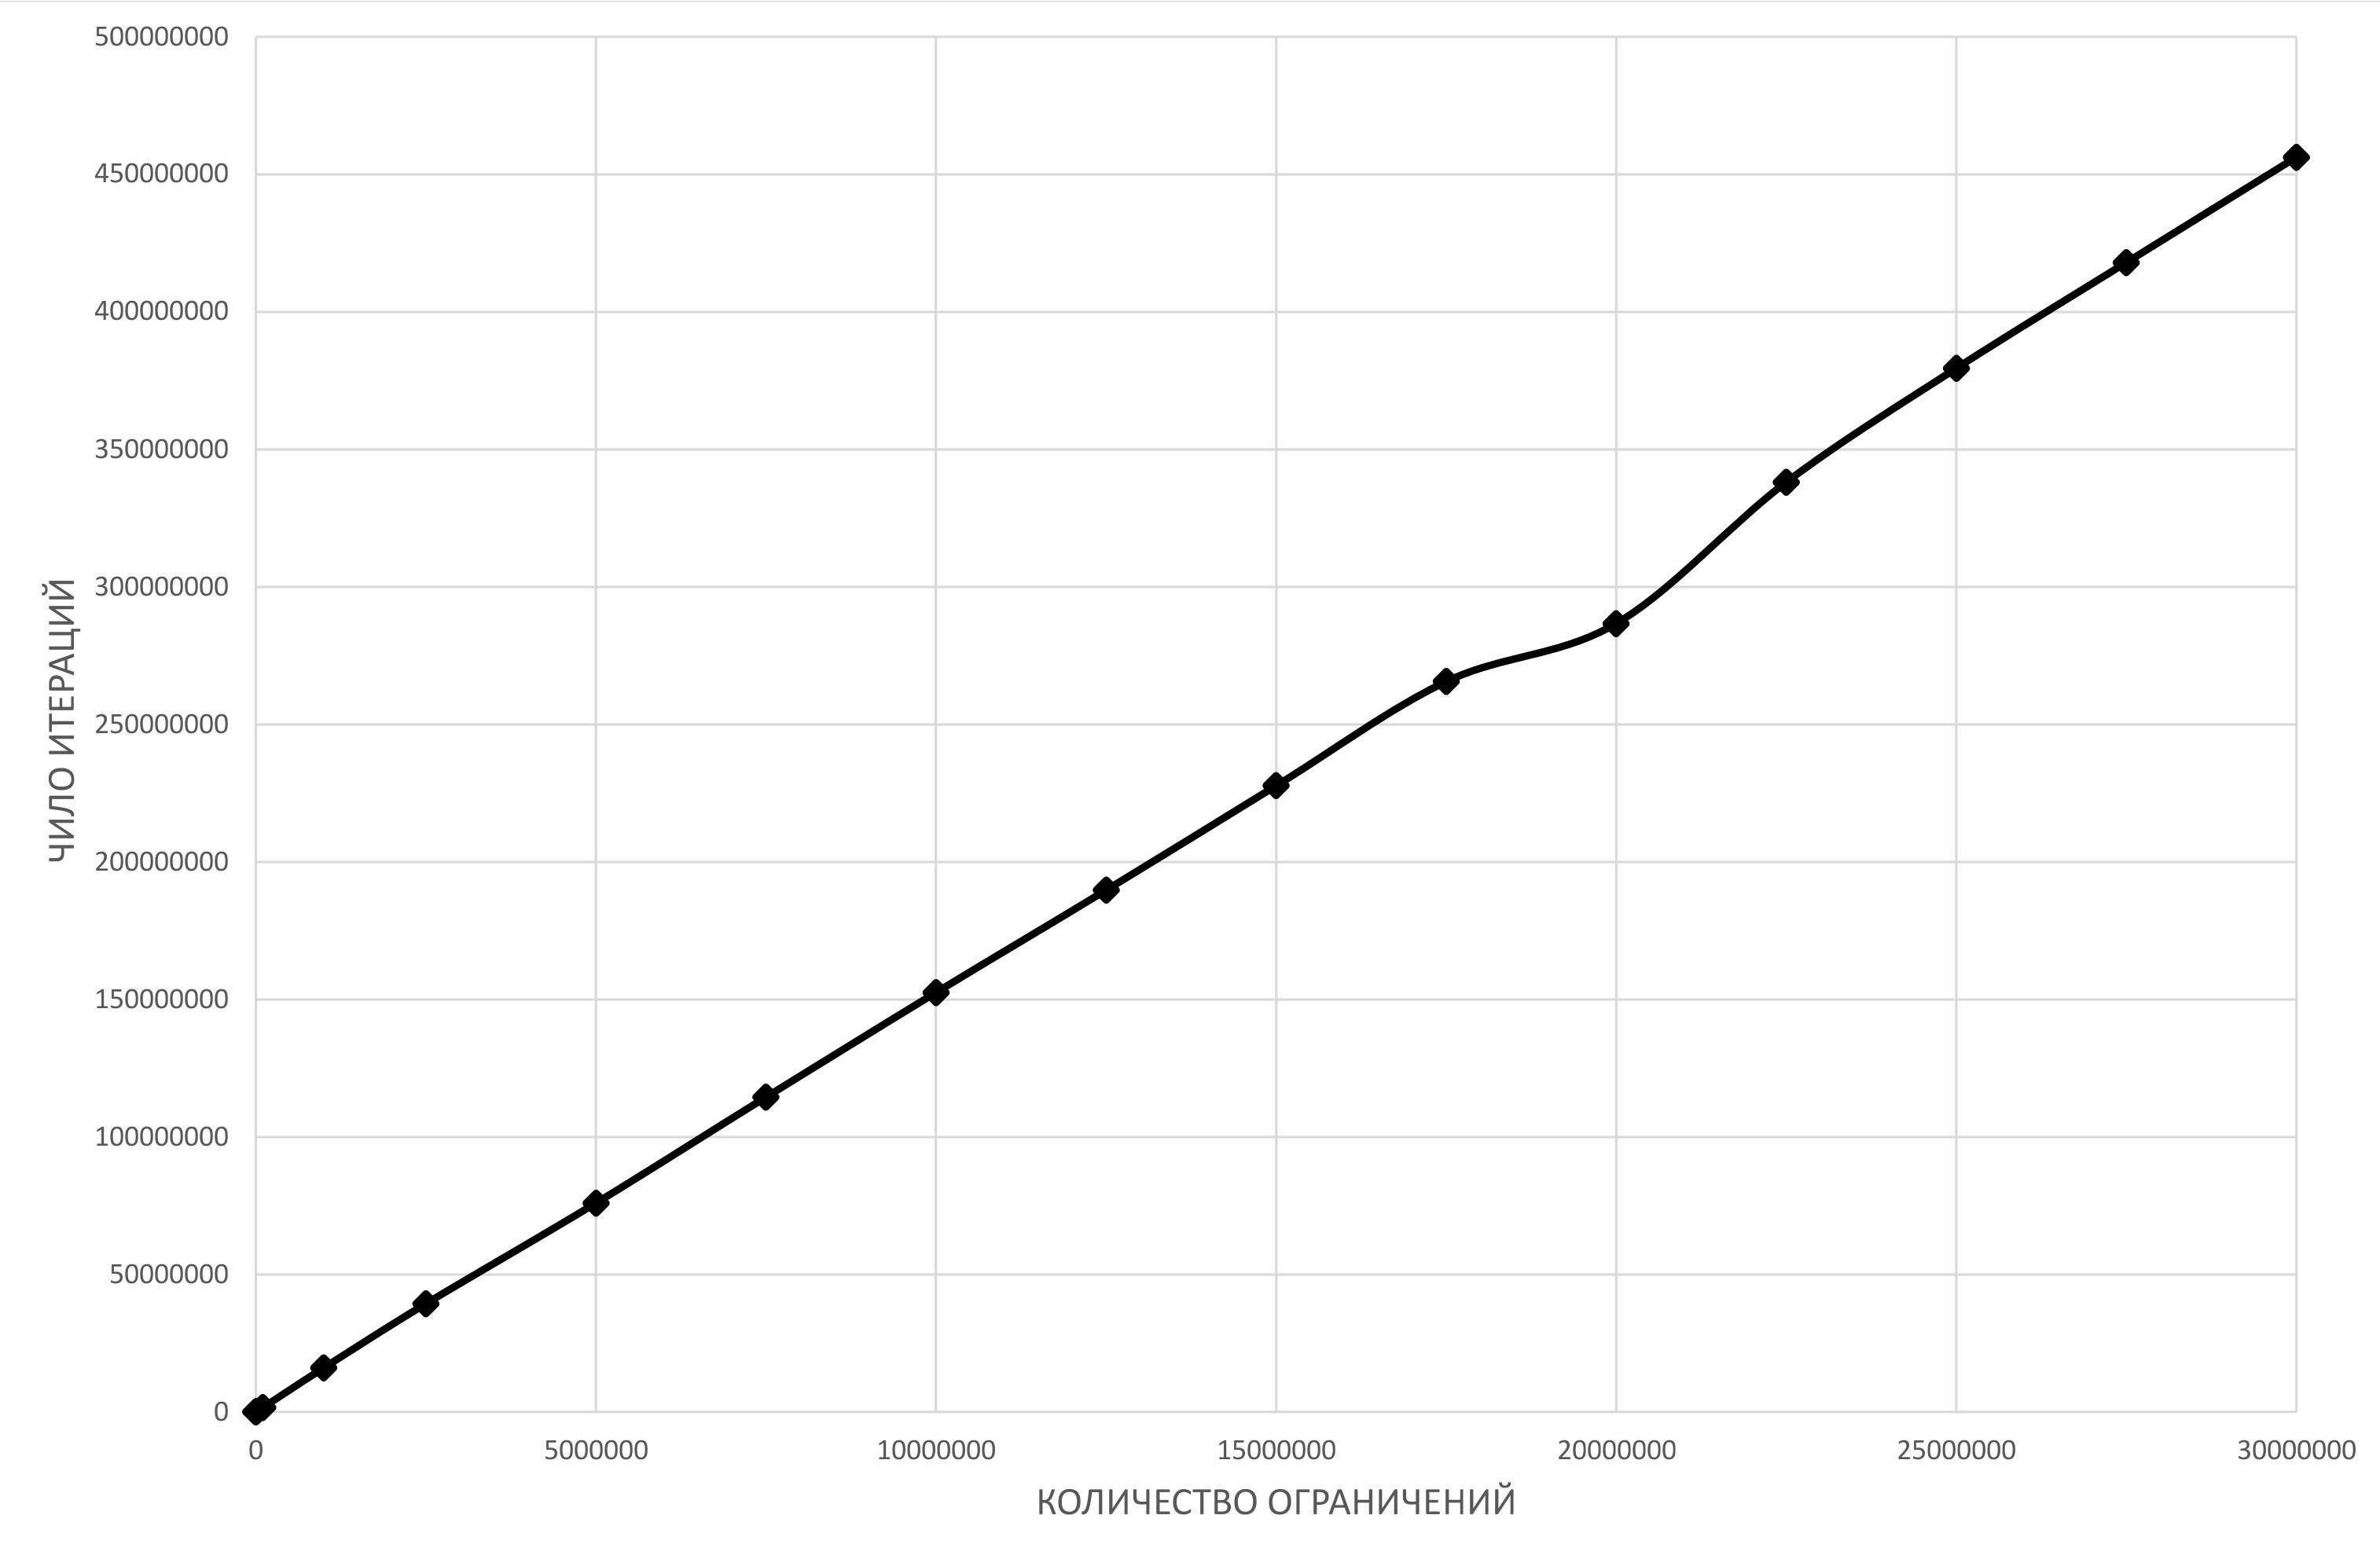
\includegraphics[width=0.9\linewidth]{Images/Meg2}}
\caption{Работа алгоритма Мегиддо.}
\label{ris:Meg2}
\end{figure}


%%%%%%%%%%%%%%%%%%%%%%%%%%%%%%%
\newpage
\section{Заключение.}
В выполненной работе были описаны и реализованы два алгоритма:
\begin{enumerate}
\item Алгоритм Мегиддо - оптимальные алгоритм решения задачи линейного программирование с двумя неизвестными. Результаты работы программной реализации алгорима соотносятся с теоритической линейной оценкой работы данного алгоритма, что является поводом утверждать, что программа была написана верно.\par
Так же получена оценка работы алгоритма $15.25m$, где m - количество ограничений.
\item Алгоритм поиска медианы - алгоритм, позволяющий отыскать медиану за линейное время и работающий, как показала практика в среднем в 40 раз быстрее алгоритма быстрой сортировки, применённого для той же цели.
\end{enumerate}
Реализация алгоритмов была произведена с использованием параллельного программирования, а именно стандарта OpenMP, а это значит что данные реализации могут быть актуальные в наше время, и способны соперничать с другими алгоритмами, решающими похожие задачи.\par
Алгоритм Мегиддо используется в алгоритме решения задачи целочисленного программирования, придуманном не так давно, в 2003 году, немецким математиком  Фридрихом Эйзенбрандом. Алгоритм Эйзенбранда способен решить задачу целочисленного программирования для двух переменных за O (m+$\phi$) арифметических операций над рациональными числами длины $\phi$, а m- количество ограничений.\par
%%%%%%%%%%%%%%%%%%%%%%%%%%%%%%%
\newpage

\begin{thebibliography}{99}
% Не удаляйте следующую строчку!
\addcontentsline{toc}{section}{Литература} 
%
\bibitem{Preparata89} Препарата, Ф., Шеймос, М. Вычислительная геометрия: Введение /  М // Мир. --- 1989. --- С. 356-365.


\bibitem{Hopk00} Хопкрофт, Дж., Ульман, Дж. , Ахо, А. Структуры данных и алгоритмы  / M. // Издательский дом "Вильямс". --- 2000. --- С. 250--264.

\bibitem{Megiddo} Megiddo, N. Linear time algorithms for linear programming in $R^{3}$ and related problems. // SIAM --- 1983. --- С. 111--130. 

\end{thebibliography}
\newpage
\appendix

\addcontentsline{toc}{section}{Приложение}
\section{Исходный код программы}

\begin{verbatim}
#include "stdafx.h"
#include "iostream"
#include <ctime>
#include <stdlib.h>
#include <math.h>
#include <omp.h>
#include <vector>
#include <algorithm>
#include <functional>
#include <iterator>


using namespace std;
int Nmax = 15;
int iter = 0;

struct Point{
	double x = 0, y = 0, tl = -1, tr = -1, 
	NumIneq1 = -1, NumIneq2 = -1, znak = 0;
};

class Inequality{
public:
	double a = 0, b = 0, c = 0;
	bool z = false;
	Inequality() {};
	Inequality(double x, double y, double p, bool q){
		a = x;
		b = y;
		c = p;
		z = q;
	}

	~Inequality() {};

	Inequality(const Inequality &X)	{
		a = X.a;
		b = X.b;
		c = X.c;
		z = X.z;
	}

	Inequality & operator= (Inequality &X){
		a = X.a;
		b = X.b;
		c = X.c;
		z = X.z;
		return (*this);
	}
	Inequality Inequality::operator/ (Inequality X)	{
		Inequality Y;
		if ((X.a != 0) && (X.b != 0) && (X.c != 0))	{
			Y.a = a / X.a;
			Y.b = b / X.b;
			Y.c = c / X.c;
		}
		return Y;
	}
	Inequality Inequality::operator+ (Inequality X)	{
		Inequality Y;
		Y.a = a + X.a;
		Y.b = b + X.b;
		Y.c = c + X.c;
		Y.z = X.z;
		return Y;
	}
	Inequality Inequality::operator- (Inequality X)	{
		Inequality Y;
		Y.a = a - X.a;
		Y.b = b - X.b;
		Y.c = c - X.c;
		Y.z = X.z;
		return Y;
	}
	friend ostream &operator<<(ostream &, Inequality &);
	friend istream &operator >> (istream &, Inequality &);
};

struct Qfunc{
	double a = 0, b = 0, c = 0;
	friend ostream &operator<<(ostream &, Qfunc &);
};

struct Lim{
	double u1 = -INFINITY;
	double u2 = +INFINITY;
};

Point PointInterseption(vector<Inequality>& A, 
	vector<int>& Index,int i,int j){
	Point X;
	X.x = -(A[Index[i]].c*A[Index[j]].b - A[Index[j]].c*A[Index[i]].b)
	 / (A[Index[i]].a*A[Index[j]].b - A[Index[j]].a*A[Index[i]].b);
	X.y = (A[Index[i]].a*A[Index[j]].c - A[Index[j]].a*A[Index[i]].c)
	 / (A[Index[i]].a*A[Index[j]].b - A[Index[j]].a*A[Index[i]].b);
	X.NumIneq1 = Index[i];
	X.NumIneq2 = Index[j];
	return X;
}
Point DeleteIneq(vector<Inequality>& A, vector<int>& IPlus,
	 vector<int>& IMinus, Lim& U);

void rand(Qfunc& Q, vector<Inequality>& A){
	Q.a = 1 + rand() % 10000;
	Q.b = 1 + rand() % 10000;
	int i = 10;
#pragma omp parallel shared (A) private (i){
		for (i = 10; i < A.size(); i++){
			A[i].a = -500 + rand() % 1000;
			A[i].b = -500 + rand() % 1000;
			A[i].c = -500 + rand() % 1000;
		}
	}
}

Point Mediana(vector<Point>& A,int q){
	Point Med;
	div_t d = div(q, 5);
#pragma omp parallel for
	for (int j = 0; j < d.quot; j++){
		for (int i = j * 5; i < (j + 1) * 5; i++){
			for (int k = 4; k > 0; k--){
				if (A[k + j * 5].x < A[k + j * 5 - 1].x)
					swap(A[k + j * 5], A[k + j * 5 - 1]);
			}
		}
		A[j] = A[j * 5 + 2];
	}
	div_t q1 = div(d.quot, 5);
	if (q1.quot != 0)
		Mediana(A,d.quot);
	else{
		for (int i = 0; i < d.quot; i++){
			for (int k = d.quot - 1; k > 0; k--){
				if (A[k].x < A[k - 1].x)
					swap(A[k], A[k - 1]);
			}
		}
		Med = A[div(d.quot, 2).quot];
		return Med;
	}
}

void Norm(Qfunc& Q, vector<Inequality>& A){
#pragma omp parallel for
	for (int i = 0; i < A.size(); i++){
		A[i].b = A[i].b / Q.b;
		A[i].a = A[i].a - A[i].b*Q.a;
	}
	Q.b = Q.b / Q.b;
	Q.a = 0;
}

void Divided(vector<Inequality>& A, vector<int>& IPlus, 
	vector<int>& IMinus, vector<int>& IZero)
{
	if (!A.empty()){
		for (int i = 0; i < A.size(); i++){
			if (A[i].b > 0){
				IPlus.push_back(i);
			}
			if (A[i].b < 0){
				IMinus.push_back(i);
			}
			if (A[i].b == 0){
				IZero.push_back(i);
			}
		}
	}
}

vector<int> FindsLimX(Lim& U, vector<Inequality>& A,
	 vector<int>& IZero){
	bool Error = false;
	if (!IZero.empty()){
		for (int i = 0; i < IZero.size(); i++){
			double del = -(A[IZero[i]].c / A[IZero[i]].a);
			if (A[IZero[i]].a < 0){
				if (del < U.u2){
					U.u2 = del;
				}
			}
			else{
				if (del > U.u1){
					U.u1 = del;
				}
			}
		}
			U.u1 = -INFINITY;
			U.u2 = +INFINITY;
	}
	return IZero;
}

void TransformationPlus(vector<Inequality>& A,
	 vector<int>& Index){
	if (!Index.empty()){
#pragma omp parallel for
		for (int i = 0; i < Index.size(); i++){
			A[Index[i]].a = -(A[Index[i]].a 
				/ A[Index[i]].b);
			A[Index[i]].c = -(A[Index[i]].c 
				/ A[Index[i]].b);
			A[Index[i]].b = 1;
		}
	}
}

void TransformationMinus(vector<Inequality>& A, 
	vector<int>& Index){
	if (!Index.empty()){
#pragma omp parallel for
		for (int i = 0; i < Index.size(); i++){
			A[Index[i]].a = -(A[Index[i]].a 
				/ A[Index[i]].b);
			A[Index[i]].c = -(A[Index[i]].c 
				/ A[Index[i]].b);
			A[Index[i]].b = 1;
		}
	}
}

Point FuncPlus(vector<Inequality>& A, vector<int>& IPlus,
	 double x){
	Point fp;
	fp.x = x;
	fp.y = INFINITY;
	if (!IPlus.empty()){
		for (int i = 0; i < IPlus.size(); i++){
			if (fp.y > (A[IPlus[i]].a*x + A[IPlus[i]].c)){
				if (abs(fp.y - (A[IPlus[i]].a*x 
					+ A[IPlus[i]].c)) < 0.000000001)
					fp.NumIneq2 = IPlus[i];
				else{
					fp.y = (A[IPlus[i]].a*x + A[IPlus[i]].c);
					fp.NumIneq1 = IPlus[i];
					continue;
				}
			}
			if (fp.y == (A[IPlus[i]].a*x + A[IPlus[i]].c))
				fp.NumIneq2 = IPlus[i];
		}
		if (fp.NumIneq2 != -1){
			if (A[fp.NumIneq1].a > A[fp.NumIneq2].a){
				fp.tl = A[fp.NumIneq1].a;
				fp.tr = A[fp.NumIneq2].a;
			}
			else{
				fp.tl = A[fp.NumIneq2].a;
				fp.tr = A[fp.NumIneq1].a;
			}
		}
		else{
			fp.tl = A[fp.NumIneq1].a;
			fp.tr = A[fp.NumIneq1].a;
		}
	}
	return fp;
}

Point FuncMinus(vector<Inequality>& A, 
	vector<int>& IMinus, double x)
{
	Point fm;
	fm.x = x;
	fm.y = -INFINITY;
	if (!IMinus.empty()){
		fm.y = -INFINITY;
		for (int i = 0; i < IMinus.size(); i++){
			if (fm.y < A[IMinus[i]].a*x + A[IMinus[i]].c){
				if (abs(fm.y - (A[IMinus[i]].a*x 
					+ A[IMinus[i]].c)) < 0.000000001)
					fm.NumIneq2 = IMinus[i];
				else{
					fm.y = (A[IMinus[i]].a*x + A[IMinus[i]].c);
					fm.NumIneq1 = IMinus[i];
				}
				continue;
			}
			if (fm.y == (A[IMinus[i]].a*x + A[IMinus[i]].c))
				fm.NumIneq2 = IMinus[i];
		}
		if (fm.NumIneq2 != -1){
			if (A[fm.NumIneq1].a < A[fm.NumIneq2].a){
				fm.tl = A[fm.NumIneq1].a;
				fm.tr = A[fm.NumIneq2].a;
			}
			else{
				fm.tl = A[fm.NumIneq2].a;
				fm.tr = A[fm.NumIneq1].a;
			}
		}
		else
		{
			fm.tl = A[fm.NumIneq1].a;
			fm.tr = A[fm.NumIneq1].a;
		}
	}
	return fm;
}

Point FindSolution(vector<Inequality>& A, vector<int>& IPlus, 
		vector<int>& IMinus, Lim& U){
	printInequality(A,IMinus);
	Point Solution;
	if((FuncMinus(A, IMinus, U.u2).y <= FuncMinus(A, IMinus, U.u1).y))
		Solution = FuncMinus(A, IMinus, U.u2);
	else
		Solution = FuncMinus(A, IMinus, U.u1);
	for (int i = 0; i < IMinus.size(); i++){
		for (int j = i + 1; j < IMinus.size(); j++){
			Point x;
			x = PointInterseption(A, IMinus, i, j);
			if ((x.x >= U.u1) && (x.x <= U.u2) && 
				(x.y < FuncPlus(A, IPlus, x.x).y))
				if (x.y < Solution.y)
					Solution = x;
		}
	}
	IPlus.clear();
	IMinus.clear();
	return Solution;
}
Point InterPointDel(vector<Inequality>& A, vector<int>& IPlus, 
		vector<int>& IMinus, Lim& U){
	vector<Point> P;
	vector<int> IPlus2;
	vector<int> IMinus2;
	Point Med, fp, fm;
	if (!IPlus.empty()){
		for (int i = 0; i < IPlus.size() - 1; i = i + 2){
			Point x;
			x = PointInterseption(A, IPlus, i, i + 1);
			x.znak = 1;
			P.push_back(x);
		}
	}
	if (!IMinus.empty()){
		for (int i = 0; i < IMinus.size() - 1; i = i + 2){
			Point x;
			x = PointInterseption(A, IMinus, i, i + 1);
			x.znak = -1;
			P.push_back(x);
		}
	}
	if (!P.empty()){
		Med = Mediana(P, P.size());
		fp = FuncPlus(A, IPlus, Med.x);
		fm = FuncMinus(A, IMinus, Med.x);
		if (fp.y < fm.y)
		{
			if (fm.tl > fp.tl)// допустимые слева
			{
				for (int i = 0; i < P.size(); i++){
					if (Med.x <= P[i].x){
						if (A[P[i].NumIneq1].a < A[P[i].NumIneq2].a){
							if (P[i].znak == -1)
								IMinus2.push_back(P[i].NumIneq1);
							if (P[i].znak == 1)
								IPlus2.push_back(P[i].NumIneq2);
						}
						else{
							if (P[i].znak == -1)
								IMinus2.push_back(P[i].NumIneq2);
							if (P[i].znak == 1)
								IPlus2.push_back(P[i].NumIneq1);
						}
					}
					else{
						if (P[i].znak == -1){
							IMinus2.push_back(P[i].NumIneq1);
							IMinus2.push_back(P[i].NumIneq2);
						}
						if (P[i].znak == 1){
							IPlus2.push_back(P[i].NumIneq1);
							IPlus2.push_back(P[i].NumIneq2);
						}
					}
				}
				U.u2 = Med.x;
			}
			if (fm.tr < fp.tr)//допустимые справа
			{
				for (int i = 0; i < P.size(); i++){
					if (Med.x >= P[i].x){
						if (A[P[i].NumIneq1].a > A[P[i].NumIneq2].a){
							if (P[i].znak == -1)
								IMinus2.push_back(P[i].NumIneq1);
							if (P[i].znak == 1)
								IPlus2.push_back(P[i].NumIneq2);
						}
						else{
							if (P[i].znak == -1)
								IMinus2.push_back(P[i].NumIneq2);
							if (P[i].znak == 1)
								IPlus2.push_back(P[i].NumIneq1);
						}
					}
					else{
						if (P[i].znak == -1){
							IMinus2.push_back(P[i].NumIneq1);
							IMinus2.push_back(P[i].NumIneq2);
						}
						if (P[i].znak == 1){
							IPlus2.push_back(P[i].NumIneq1);
							IPlus2.push_back(P[i].NumIneq2);
						}
					}
				}
				U.u1 = Med.x;
			}
			if ((fm.tl <= fp.tl) || (fm.tr >= fp.tr))//неразрешима
			{
				cout << "Задача не разрешима" << endl;
			}
		}
		else{
			if ((fm.tr >= fm.tl) && (fm.tr > 0) 
				&& (fm.tl > 0))// минимум слева
			{
				for (int i = 0; i < P.size(); i++){
					if (Med.x <= P[i].x){
						if (A[P[i].NumIneq1].a < A[P[i].NumIneq2].a){
							if (P[i].znak == -1)
								IMinus2.push_back(P[i].NumIneq1);
							if (P[i].znak == 1)
								IPlus2.push_back(P[i].NumIneq2);
						}
						else{
							if (P[i].znak == -1)
								IMinus2.push_back(P[i].NumIneq2);
							if (P[i].znak == 1)
								IPlus2.push_back(P[i].NumIneq1);
						}
					}
					else{
						if (P[i].znak == -1){
							IMinus2.push_back(P[i].NumIneq1);
							IMinus2.push_back(P[i].NumIneq2);
						}
						if (P[i].znak == 1){
							IPlus2.push_back(P[i].NumIneq1);
							IPlus2.push_back(P[i].NumIneq2);
						}
					}
				}
				U.u2 = Med.x;
			}
			if ((fm.tl <= fm.tr) && (fm.tr < 0) 
				&& (fm.tl < 0))// минимум справа
			{
				for (int i = 0; i < P.size(); i++){
					if (Med.x >= P[i].x){
						if (A[P[i].NumIneq1].a > A[P[i].NumIneq2].a){
							if (P[i].znak == -1)
								IMinus2.push_back(P[i].NumIneq1);
							if (P[i].znak == 1)
								IPlus2.push_back(P[i].NumIneq2);
						}
						else{
							if (P[i].znak == -1)
								IMinus2.push_back(P[i].NumIneq2);
							if (P[i].znak == 1)
								IPlus2.push_back(P[i].NumIneq1);
						}
					}
					else{
						if (P[i].znak == -1){
							IMinus2.push_back(P[i].NumIneq1);
							IMinus2.push_back(P[i].NumIneq2);
						}
						if (P[i].znak == 1){
							IPlus2.push_back(P[i].NumIneq1);
							IPlus2.push_back(P[i].NumIneq2);
						}
					}
				}
				U.u1 = Med.x;
			}
			if ((fm.tl < 0) && (fm.tr > 0)){
				cout << "Минимум достигается в точке" << fm << endl;
				return fm;
			}
		}
	}
	IPlus.clear();
	IPlus = IPlus2;
	IPlus2.clear();
	IMinus.clear();
	IMinus = IMinus2;
	IMinus2.clear();
}
Point DeleteIneq(vector<Inequality>& A, vector<int>& IPlus, 
		vector<int>& IMinus, Lim& U){
	vector<int> IPlus2;
	vector<int> IPlus3;
	vector<int> IMinus2;
	vector<int> IMinus3;
#pragma omp parallel sections{
#pragma omp section{		
			if (!IPlus.empty()){
				if (IPlus.size() & 1)
					IPlus2.push_back(IPlus[IPlus.size() - 1]);
				for (int i = 0; i < IPlus.size() - 1; i = i + 2){
					if (A[IPlus[i]].a == A[IPlus[i + 1]].a){
						if (A[IPlus[i]].c > A[IPlus[i + 1]].c)
							IPlus2.push_back(IPlus[i + 1]);
						else
							IPlus2.push_back(IPlus[i]);
					}
					else{
						Point X = PointInterseption(A, IPlus, i, i + 1);
						if (X.x < U.u1){
							if (A[IPlus[i]].a > A[IPlus[i + 1]].a)
								IPlus2.push_back(IPlus[i + 1]);
							else
								IPlus2.push_back(IPlus[i]);
						}
						if (X.x > U.u2){
							if (A[IPlus[i]].a > A[IPlus[i + 1]].a)
								IPlus2.push_back(IPlus[i]);
							else
								IPlus2.push_back(IPlus[i + 1]);
						}
						if ((U.u1 <= X.x) && (X.x <= U.u2)){
							IPlus3.push_back(IPlus[i]);
							IPlus3.push_back(IPlus[i + 1]);
						}
					}
				}
				IPlus.clear();
				IPlus = IPlus2;
				IPlus2.clear();
			}
		}
#pragma omp section{
			if (!IMinus.empty()){
				if (IMinus.size() & 1)
					IMinus2.push_back(IMinus[IMinus.size() - 1]);
				for (int i = 0; i < IMinus.size() - 1; i = i + 2){
					if (A[IMinus[i]].a == A[IMinus[i + 1]].a){
						if (A[IMinus[i]].c < A[IMinus[i + 1]].c)
							IMinus2.push_back(IMinus[i]);
						else
							IMinus2.push_back(IMinus[i + 1]);
					}
					else{
						Point X = PointInterseption(A, IMinus, i, i + 1);
						if (X.x < U.u1){
							if (A[IMinus[i]].a > A[IMinus[i + 1]].a)
								IMinus2.push_back(IMinus[i]);
							else
								IMinus2.push_back(IMinus[i + 1]);
						}
						if (X.x > U.u2){
							if (A[IMinus[i]].a > A[IMinus[i + 1]].a)
								IMinus2.push_back(IMinus[i + 1]);
							else
								IMinus2.push_back(IMinus[i]);
						}
						if ((U.u1 <= X.x) && (X.x <= U.u2)){
							IMinus3.push_back(IMinus[i]);
							IMinus3.push_back(IMinus[i + 1]);
						}
					}
				}
				IMinus.clear();
				IMinus = IMinus2;
				IMinus2.clear();
			}
		}
	}
#pragma omp barrier 
	if (IPlus.size() + IMinus.size()+
			IMinus3.size()+IPlus3.size() > 10){
		InterPointDel(A, IPlus3, IMinus3, U);
		for (int i = 0; i < IPlus3.size(); i++)
			IPlus.push_back(IPlus3[i]);
		for (int i = 0; i < IMinus3.size(); i++)
			IMinus.push_back(IMinus3[i]);
		IPlus3.clear();
		IMinus3.clear();
		return DeleteIneq(A, IPlus, IMinus, U);
	}
	else
		return FindSolution(A, IPlus, IMinus, U);
}
void CreateExample(vector<Inequality>& A){
	int R=500;
	for (int i = 0; i < A.size(); i++){
		double x1, x2, y1, y2;
		x1 = rand() % R + (-R);
		if (x1 > 0){
			x2 = rand() % R;
			y1 = -sqrt(R*R - x1*x1);
			y2 = -sqrt(R*R - x2*x2);
		}
		else{
			x2 = rand() % -R + 0;
			y1 = -sqrt(R*R - x1*x1);
			y2 = -sqrt(R*R - x2*x2);
		}
		A[i].a = y1 - y2;
		A[i].b = -x2 + x1;
		A[i].c = x1*y2 - x2*y1;
	}
}

int main(){
	vector<Inequality> A(n);
	vector<int> IPlus,IMinus,IZero;
	Lim U;
	Qfunc Q;
	Q.a = 6; Q.b = 7; Q.c = 0;
	CreateExample(A);
	printInequality(Q, A);
	Norm(Q, A);
	Divided(A, IPlus, IMinus, IZero);// разделение на 3 класса
	IZero = FindsLimX(U, A, IZero);
	TransformationPlus(A, IPlus);
	TransformationMinus(A, IMinus);
	Point Solution;
	Solution = DeleteIneq(A, IPlus, IMinus, U);
	IPlus.clear();
	IMinus.clear();
	IZero.clear();
	A.clear();
	cout << "Решение = " << Solution << endl;
	cout << "Время = " << te - ts << endl;
	cout << "Количество итераций = " << iter << endl;
	iter = 0;
	system("pause");
	return 0;
}
\end{verbatim}
\end{document}